\documentclass[a4paper,zihao=-4]{article}

%---------------------------------------------------------------------------------
% 宏包引入
%---------------------------------------------------------------------------------
\usepackage[UTF8, heading=true, scheme=chinese]{ctex} % 中文支持
\usepackage{geometry}       % 页面设置
\usepackage{amsmath, amssymb} % 数学公式
\usepackage{graphicx}       % 图片支持
\usepackage{fontspec}       % 字体设置
\usepackage{titlesec}       % 标题格式定制
\usepackage{fancyhdr}       % 页眉页脚
\usepackage{setspace}       % 行距设置
\usepackage{caption}        % 图表标题设置
\usepackage{booktabs}       % 表格美化
\usepackage{float}          % 浮动体位置固定
\usepackage{titling}        % 标题宏包
\usepackage{times}          % 设置英文为Times New Roman
\usepackage{ulem}           % 提供下划线功能

\usepackage{url}          % 基础URL处理
\usepackage{xurl}         % 支持URL任意位置自动分行（XeLaTeX首选）
\usepackage{hyperref}     % 可选：让URL可点击（不影响分行）

\usepackage{ragged2e}     % 优化对齐，避免字间距异常



%---------------------------------------------------------------------------------
% 页面与字体设置 (Strictly following the Word template)
%---------------------------------------------------------------------------------

% 1. 版式说明：A4纸，页边距一般默认2.5cm
\geometry{left=2.5cm, right=2.5cm, top=2.5cm, bottom=2.5cm}

% 2. 页眉页脚设置
% 清空所有页眉页脚设置
\fancyhf{}
% 设置页码在页脚中央
\fancyfoot[C]{\thepage}
% 设置页眉和页脚线的宽度为0（不显示）
\renewcommand{\headrulewidth}{0pt}
\renewcommand{\footrulewidth}{0pt}
% 应用设置到所有页面
\pagestyle{fancy}

% 2. 字体设置
% 正文：宋体小4号 (ctex默认zihao=-4即为小四)
% 英文：Times New Roman 小4号
\setmainfont{Times New Roman}
\setCJKmainfont[AutoFakeBold=true]{SimSun} % 指定宋体，并允许伪粗体

% 3. 行间距：全文统一 1.5倍
\onehalfspacing

% 4. 标题格式设置
% 一级标题：宋体三号加黑，居中 (使用黑体模拟加黑的宋体效果，通常报告用黑体更正式，若必须宋体加粗可改 \songti\bfseries)
% 模版要求：一级标题用宋体三号加黑，居中。这里使用黑体对应"加黑"视觉效果，符合常规排版习惯。
\ctexset{
	section = {
		format = \centering\bfseries\zihao{3}, % 三号加黑 居中
		name = {,},
		number = \arabic{section},
		aftername = \quad
	},
	subsection = {
		format = \raggedright\bfseries\zihao{4}, % 四号加黑 左对齐
		name = {,},
		number = \arabic{section}.\arabic{subsection},
		aftername = \quad
	},
	subsubsection = {
		format = \raggedright\bfseries\zihao{-4}, % 小四号加黑 左对齐
		name = {,},
		number = \arabic{section}.\arabic{subsection}.\arabic{subsubsection},
		aftername = \quad
	}
}

% 5. 图表标题设置
% 图表用宋体5号字
\DeclareCaptionFont{songtiFive}{\songti\zihao{5}}
\captionsetup{
	font=songtiFive,
	labelsep=quad, % 序号和标题间空一格
	labelfont=bf,  % 序号加粗
	textfont=normalfont
}
% 公式序号右对齐（默认），按章编号
\numberwithin{equation}{section}
% 图表按章编号
\numberwithin{figure}{section}
\numberwithin{table}{section}

%---------------------------------------------------------------------------------
% 文档开始
%---------------------------------------------------------------------------------
\begin{document}
	
	%---------------------------------------------------------------------------------
	% 封面页
	%---------------------------------------------------------------------------------
	\begin{titlepage}
		\centering
		\vspace*{2cm}
		
		{\zihao{1}\bfseries 综合课程设计报告\par}
		
		\vspace{3cm}
		
		{\zihao{2}\bfseries 设计题目：控制理论与方法课程设计\par}
		
		\vspace{3cm}
		
		{\zihao{3}
			\begin{tabular}{c}
				姓名-班级-学号：\\
				同学B-强基班-学号-比例：60\% \\
				匿名-强基班-学号-比例：40\% \\
			\end{tabular}\par}
		
		\vspace{2cm}
		
		{\zihao{3}
			\begin{tabular}{c}
				指导教师：匿名\\
			\end{tabular}\par}
		
		\vspace{2cm}
		
		{\zihao{3}
			\begin{tabular}{c}
				设计时间：2025.12.2-2025.1.8\\
			\end{tabular}\par}
		
		\vfill
	\end{titlepage}
	
	%---------------------------------------------------------------------------------
	% 目录
	%---------------------------------------------------------------------------------
	\newpage
	\pagenumbering{Roman} % 目录页用罗马数字
	\tableofcontents
	\newpage
	
	%---------------------------------------------------------------------------------
	% 正文主体
	%---------------------------------------------------------------------------------
	\pagenumbering{arabic} % 正文用阿拉伯数字
	\setcounter{page}{1}
	
	% 根据模版，正文首字符空两个汉字 (ctex默认已开启indentfirst)	
	\section{机械手控制系统综合设计}
	\subsection{系统闭环传递函数的建立}
	
	根据机械手控制系统结构图（图4）及题目描述，本系统为一个典型的负反馈控制系统。为了分析系统的动态性能，首先需要建立系统的数学模型。根据已知参数，系统的转动惯量 $J=0.1$，摩擦系数 $f=1$，电机增益 $K_m=30$，电阻 $R_f=1$。在第一部分分析中，假设电位计系数 $K_1=1$ 且反馈系数 $K_f=1$。
	
	\subsubsection{前向通道传递函数}
	
	系统的前向通道传递函数 $G(s)$ 由功率放大器、中间环节以及电机负载模型串联而成。将已知参数代入，可得前向传递函数为：
	\begin{equation}
		G(s) = K_1 \cdot K_2 \cdot \frac{K_m}{R_f} \cdot \frac{1}{s(Js+f)} = 1 \cdot K_2 \cdot \frac{30}{1} \cdot \frac{1}{s(0.1s+1)} = \frac{300K_2}{s(s+10)}
	\end{equation}
	
	\subsubsection{闭环传递函数与特征方程}
	
	由于系统为单位负反馈结构（$H(s)=1$），其闭环传递函数 $\Phi(s)$ 定义为输出 $\theta(s)$ 与输入 $\theta_d(s)$ 之比，计算如下：
	\begin{equation}
		\Phi(s) = \frac{G(s)}{1+G(s)H(s)} = \frac{\frac{300K_2}{s(s+10)}}{1 + \frac{300K_2}{s(s+10)}} = \frac{300K_2}{s^2 + 10s + 300K_2}
	\end{equation}
	由此可得系统的闭环特征方程为：
	\begin{equation}
		D(s) = s^2 + 10s + 300K_2 = 0
		\label{eq:char_eq}
	\end{equation}
	
	\subsubsection{基于劳斯判据的稳定性分析}
	
	为了判断系统的稳定性，我们需要依据劳斯代数判据（Routh-Hurwitz Stability Criterion）对特征方程（\ref{eq:char_eq}）进行分析。劳斯判据指出，线性系统稳定的充要条件是劳斯表中第一列的所有系数均大于零，且不发生符号改变。
	
	针对本二阶系统，我们列出如下劳斯表（Routh Array）：
	
	\begin{table}[H]
		\centering
		\caption{系统劳斯表} % 添加表标题
		\renewcommand{\arraystretch}{1.5}
		\begin{tabular}{c|cc}
			\toprule
			$s^2$ & $1$ & $300K_2$ \\
			$s^1$ & $10$ & $0$ \\
			$s^0$ & $b_1$ & \\
			\bottomrule
		\end{tabular}
	\end{table}
	
	其中，$s^0$ 行的第一列系数 $b_1$ 计算如下：
	\begin{equation}
		b_1 = \frac{10 \times 300K_2 - 1 \times 0}{10} = 300K_2
	\end{equation}
	根据劳斯判据的稳定性条件，劳斯表第一列的元素必须全部为正数。已知前两行第一列系数 $1$ 和 $10$ 恒为正，因此系统稳定的条件取决于第三行系数：
	\begin{equation}
		300K_2 > 0 \implies K_2 > 0
	\end{equation}
	综上所述，只要功率放大器的增益 $K_2$ 为正值，该机械手控制系统即为稳定系统。这与二阶系统稳定性结论一致，即特征方程所有系数均为正数时系统稳定。
	
	\subsection{单位阶跃响应求解 ($K_2=20$)}
	
	\subsubsection{阶跃响应求解}
	当功率放大器增益设定为 $K_2=20$ 时 ，将其代入闭环传递函数 $\Phi(s)$，系统变为：
	\begin{equation}
		\Phi(s) = \frac{300 \times 20}{s^2 + 10s + 300 \times 20} = \frac{6000}{s^2 + 10s + 6000}
	\end{equation}
	此时，输入信号 $\theta_d(t)$ 为单位阶跃信号，即 $\Theta_d(s) = \frac{1}{s}$ 。
	
	为了求解时域响应 $\theta(t)$，我们首先分析系统的阻尼特性。对比标准二阶系统特征方程 $s^2 + 2\zeta\omega_n s + \omega_n^2 = 0$，可得自然频率 $\omega_n$ 和阻尼比 $\zeta$：
	\begin{equation}
		\omega_n^2 = 6000 \implies \omega_n = \sqrt{6000} = 20\sqrt{15} \approx 77.46 \, \text{rad/s}
	\end{equation}
	\begin{equation}
		2\zeta\omega_n = 10 \implies \zeta = \frac{10}{2\times 77.46} \approx 0.0645
	\end{equation}
	由于 $0 < \zeta < 1$，系统处于欠阻尼状态，其阶跃响应将表现为衰减振荡过程。
	
	系统的输出在复频域表示为：
	\begin{equation}
		\Theta(s) = \Phi(s) \cdot \frac{1}{s} = \frac{6000}{s(s^2 + 10s + 6000)}
	\end{equation}
	利用拉普拉斯逆变换， 结合二阶系统的单位阶跃响应公式
	\begin{equation*}
		\theta(t) = 1 - \frac{e^{-\zeta\omega_n t}}{\sqrt{1-\zeta^2}} \sin\big(\omega_n\sqrt{1-\zeta^2} t + arctan(\frac{\sqrt{1-\zeta^2}}{\zeta})\big), \quad t \geq 0
	\end{equation*}
	该系统的单位阶跃响应为：
	\begin{equation}
		\theta(t) \approx 1 - 1.002e^{-5t} \sin(77.3t + 1.505), \quad t \geq 0
	\end{equation}
	该结果表明，系统在收到阶跃信号后，将以约 $77.3 \, \text{rad/s}$ 的频率进行振荡，并以 $e^{-5t}$ 的速率收敛至目标位置。
	
	\subsubsection{仿真验证}
	我们利用Python进行了2000个时间步的仿真验证，结果如图\ref{fig:1R}、\ref{fig:1E}:
	\begin{figure}[H]
		\centering
		% 注意：你需要确保工作目录下有名为 Bode.png 的图片文件
		% 否则请注释掉下面一行，使用 framebox 替代
		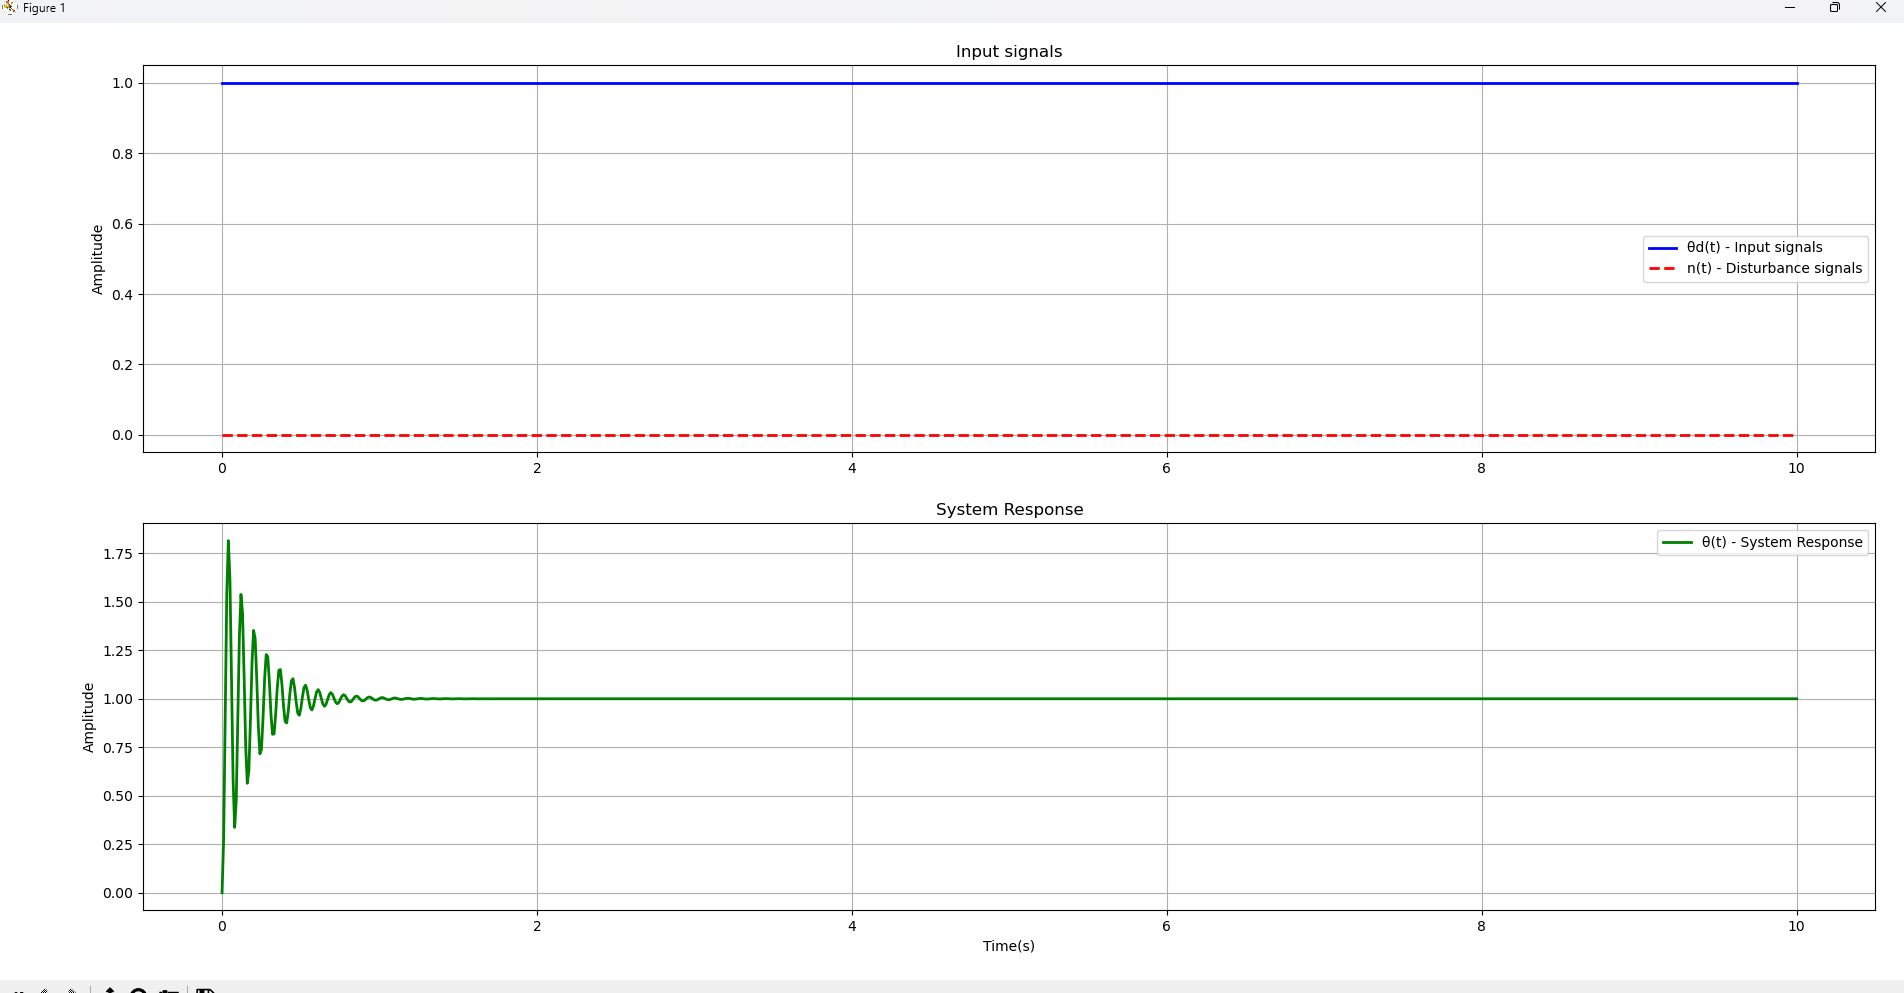
\includegraphics[width=0.8\linewidth]{1.1.png}
		\caption{系统响应曲线}
		\label{fig:1R}
	\end{figure}
	\begin{figure}[H]
		\centering
		% 注意：你需要确保工作目录下有名为 Bode.png 的图片文件
		% 否则请注释掉下面一行，使用 framebox 替代
		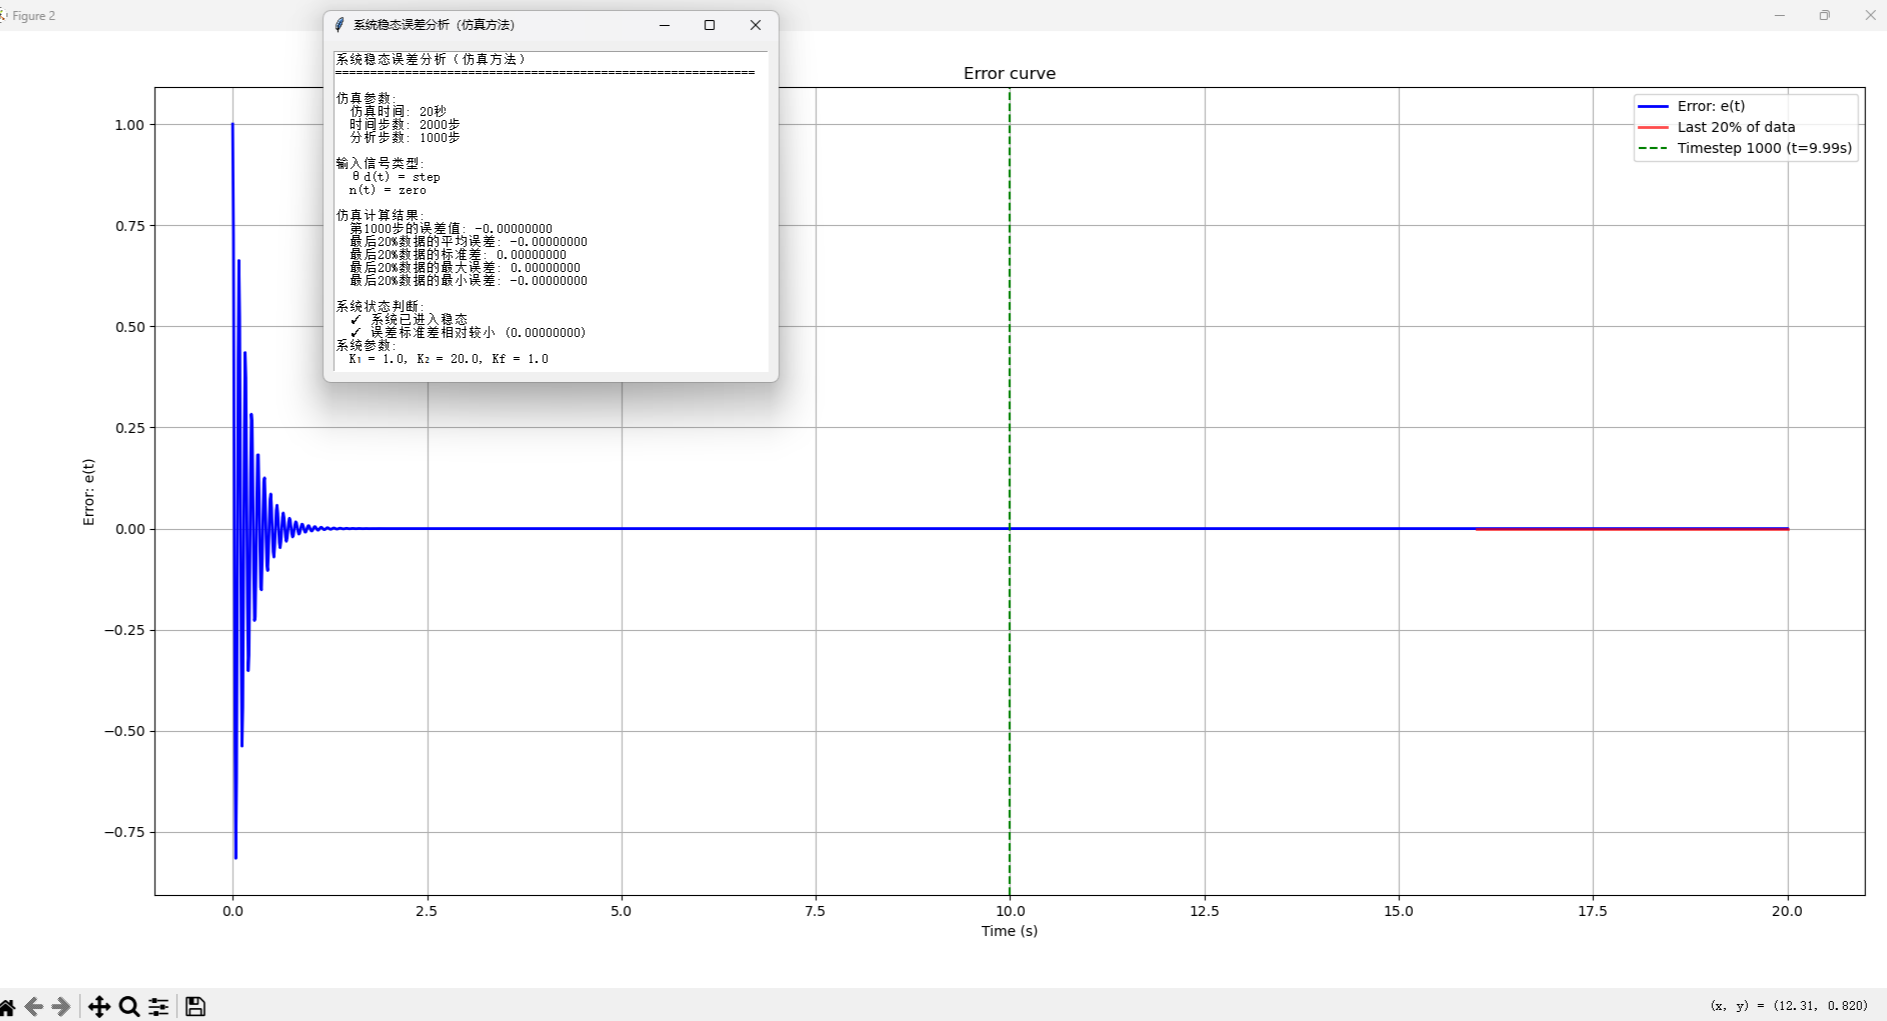
\includegraphics[width=0.8\linewidth]{1.2.png}
		\caption{误差曲线}
		\label{fig:1E}
	\end{figure}
	
	结合图中信息可知，该系统确实如上所述，稳定且衰减震荡。
	
	\subsection{稳态误差分析}
	
	题目要求确定当干扰 $n(t)=0$，输入 $\theta_d(t)=t$（单位斜坡信号）时系统的稳态误差。假设系统保持单位负反馈结构，即 $K_1=K_f=1$。
	
	\subsubsection{稳态误差的推导与计算}
	
	已知输入信号 $\theta_d(t)=t$，其拉普拉斯变换为：
	\begin{equation}
		\Theta_d(s) = \frac{1}{s^2}
	\end{equation}
	
	对于单位负反馈系统，误差信号 $E(s)$ 的表达式为：
	\begin{equation}
		E(s) = \Theta_d(s) - \theta(s) = \frac{1}{1+G(s)}\Theta_d(s)
	\end{equation}
	
	根据终值定理，系统的稳态误差 $e_{ss}$ 可以通过下式计算：
	\begin{equation}
		e_{ss} = \lim_{t \to \infty} e(t) = \lim_{s \to 0} s E(s) = \lim_{s \to 0} s \cdot \frac{1}{1+G(s)} \cdot \frac{1}{s^2} = \lim_{s \to 0} \frac{1}{s + sG(s)}
	\end{equation}
	
	将前向通道传递函数 $G(s) = \frac{300K_2}{s(s+10)}$ 代入上式中分母的 $sG(s)$ 部分进行计算：
	\begin{equation}
		\lim_{s \to 0} s G(s) = \lim_{s \to 0} s \cdot \frac{300K_2}{s(s+10)} = \lim_{s \to 0} \frac{300K_2}{s+10} = \frac{300K_2}{10} = 30K_2
	\end{equation}
	
	因此，系统的稳态误差表达式为：
	\begin{equation}
		e_{ss} = \frac{1}{0 + 30K_2} = \frac{1}{30K_2}
	\end{equation}
	
	\subsubsection{计算结果}
	
	根据上述推导，系统的稳态误差与功率放大器增益 $K_2$ 成反比。
	
	若沿用第一问中给定的增益参数 $K_2=20$，则本系统的稳态误差具体数值为：
	\begin{equation}
		e_{ss} = \frac{1}{30 \times 20} = \frac{1}{600} \approx 0.00167
	\end{equation}
	
	可知当输入为单位斜坡信号时，系统的稳态误差为 $\frac{1}{30K_2}$。在 $K_2=20$ 的条件下，稳态误差为 $0.00167 rad$ 。
	
	\subsubsection{仿真验证}
	我们利用Python进行了2000时间步的仿真验证，结果如图\ref{fig:2R}、\ref{fig:2E}:
	\begin{figure}[H]
		\centering
		% 注意：你需要确保工作目录下有名为 Bode.png 的图片文件
		% 否则请注释掉下面一行，使用 framebox 替代
		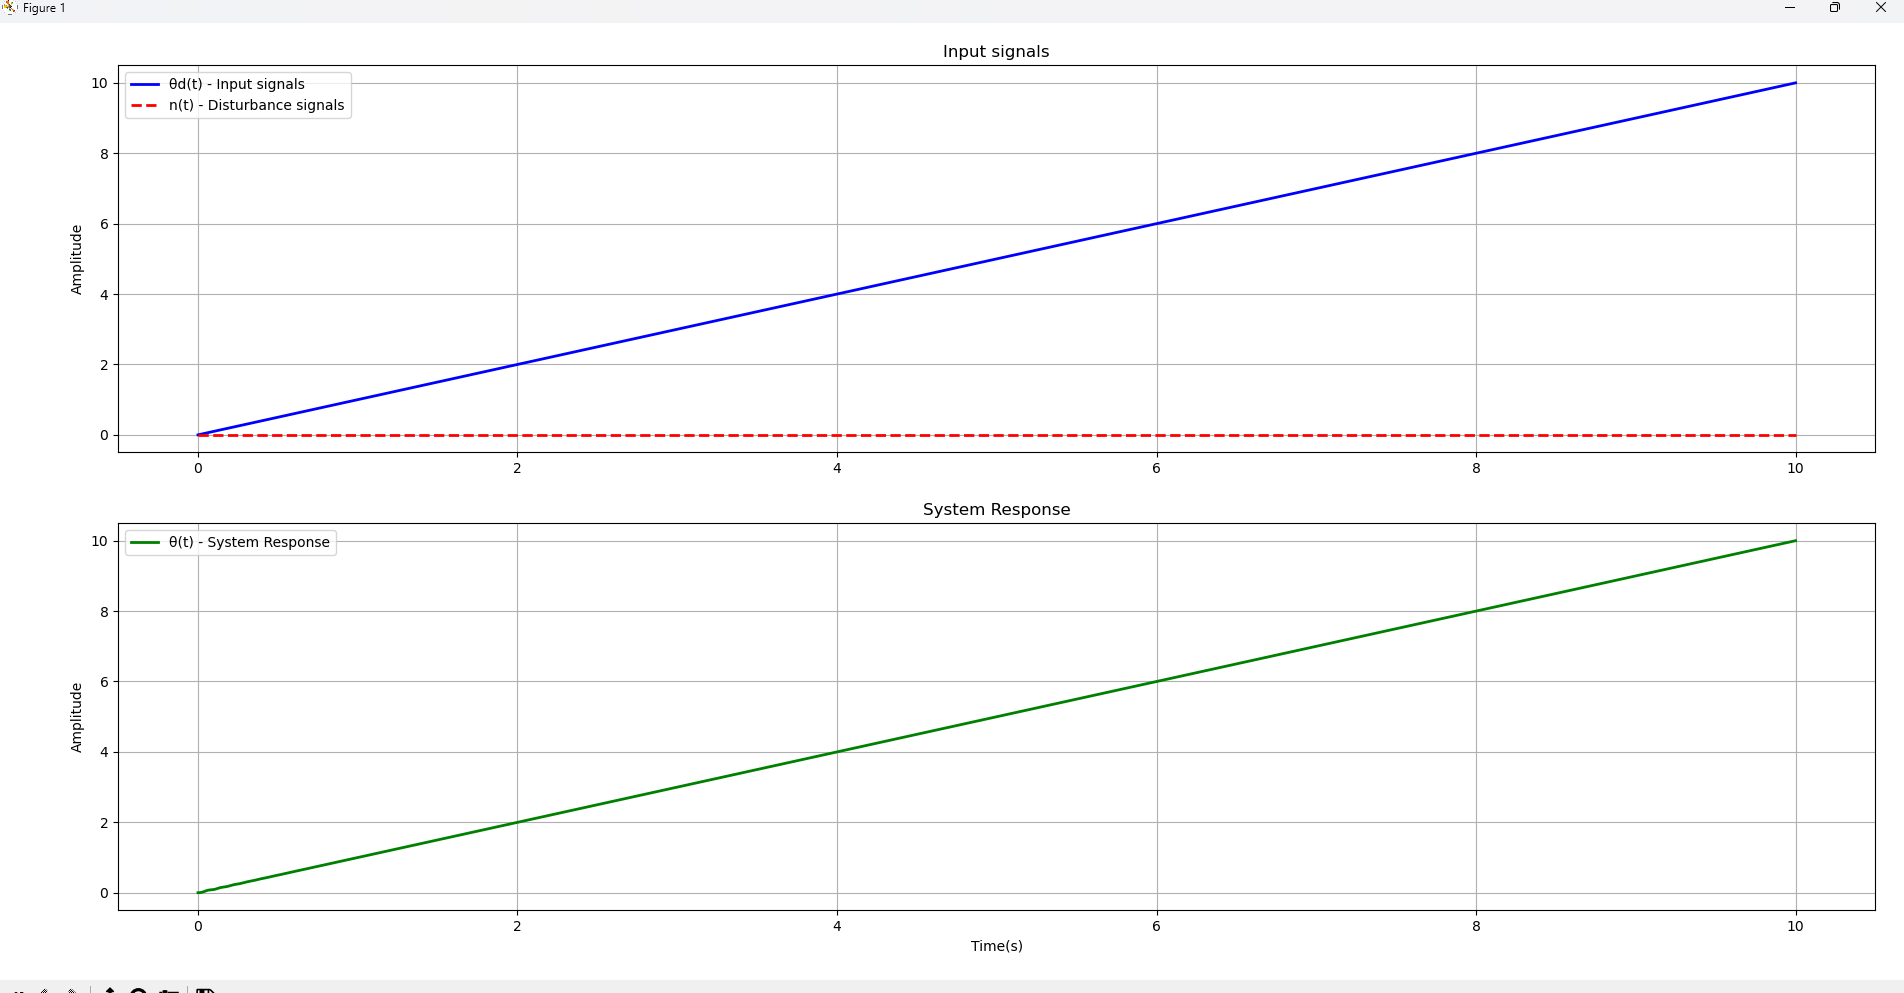
\includegraphics[width=0.8\linewidth]{2.1.png}
		\caption{系统响应曲线}
		\label{fig:2R}
	\end{figure}
	\begin{figure}[H]
		\centering
		% 注意：你需要确保工作目录下有名为 Bode.png 的图片文件
		% 否则请注释掉下面一行，使用 framebox 替代
		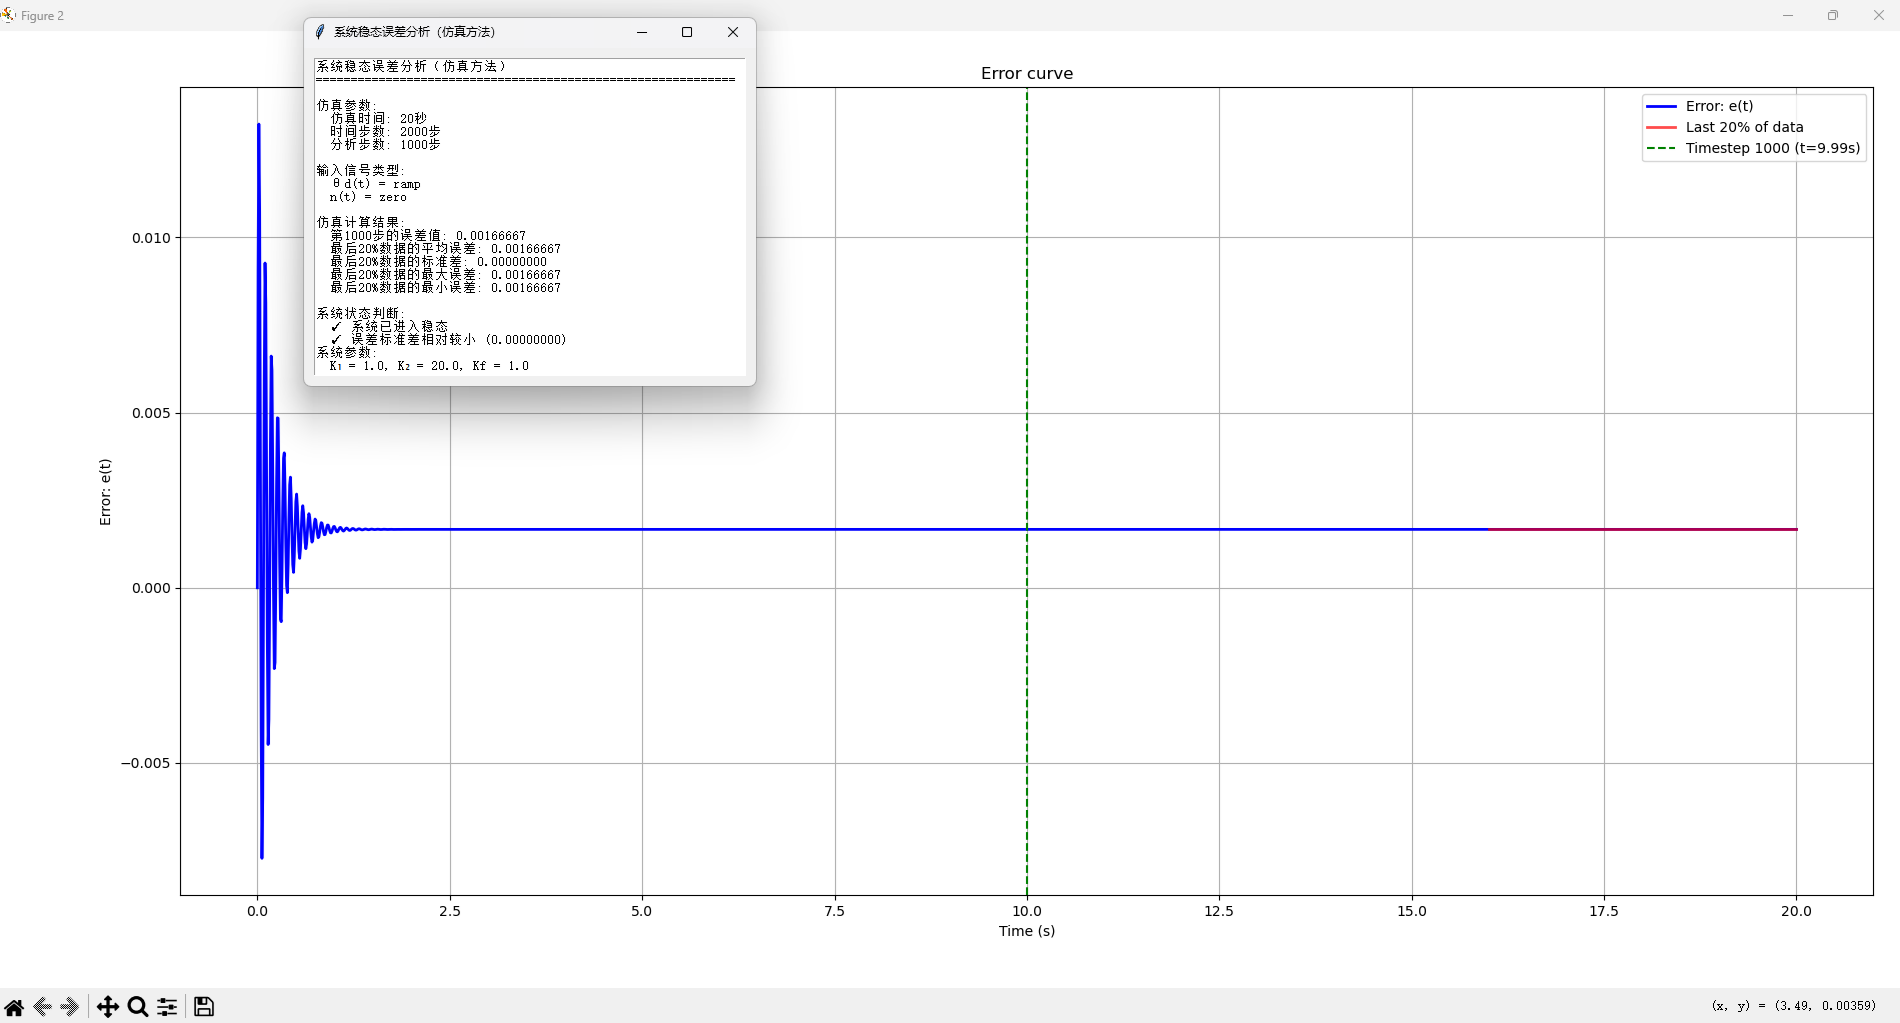
\includegraphics[width=0.8\linewidth]{2.2.png}
		\caption{误差曲线}
		\label{fig:2E}
	\end{figure}
	
	结合图中信息可知，该系统确实如上所述，在运行很长一段时间进入稳态后存在一个很小的稳态误差。
	
	\subsection{PID控制器设计与频域分析}
	
	本部分要求在不考虑前置滤波器 $G_p(s)$ 的情况下，分析引入 PID 控制器 $G_c(s)$ 后的系统开环频率特性及稳定性。
	
	\subsubsection{系统开环传递函数的建立}
	
	根据系统结构图（pdf中的图5）及参数说明，被控对象传递函数为 $G_0(s) = \frac{1}{s(s^2+4s+5)}$，PID 控制器传递函数为 $G_c(s) = \frac{4(s+1.25)^2}{s}$。
	
	此时，系统的开环传递函数 $G_{open}(s)$ 为控制器与被控对象的串联：
	\begin{equation}
		\begin{aligned}
			G_{open}(s) &= G_c(s) \cdot G_0(s) \\
			&= \frac{4(s+1.25)^2}{s} \cdot \frac{1}{s(s^2+4s+5)} \\
			&= \frac{4(s^2 + 2.5s + 1.5625)}{s^2(s^2 + 4s + 5)}
		\end{aligned}
	\end{equation}
	
	观察上式可知，分母中包含 $s^2$，说明该系统为 \textbf{II 型系统}。在低频段，其幅频特性曲线的斜率为 $-40\text{dB/dec}$，且初始相位由 $-180^\circ$ 开始。分子中的两个重零点 $s = -1.25$ 将引入相位超前，有助于提高系统的相位裕度。
	
	\subsubsection{Bode 图绘制与稳定性分析}
	
	利用 MATLAB 绘制该系统的开环 Bode 图，如图 \ref{fig:bode} 所示。
	
	\begin{figure}[H]
		\centering
		% 注意：你需要确保工作目录下有名为 Bode.png 的图片文件
		% 否则请注释掉下面一行，使用 framebox 替代
		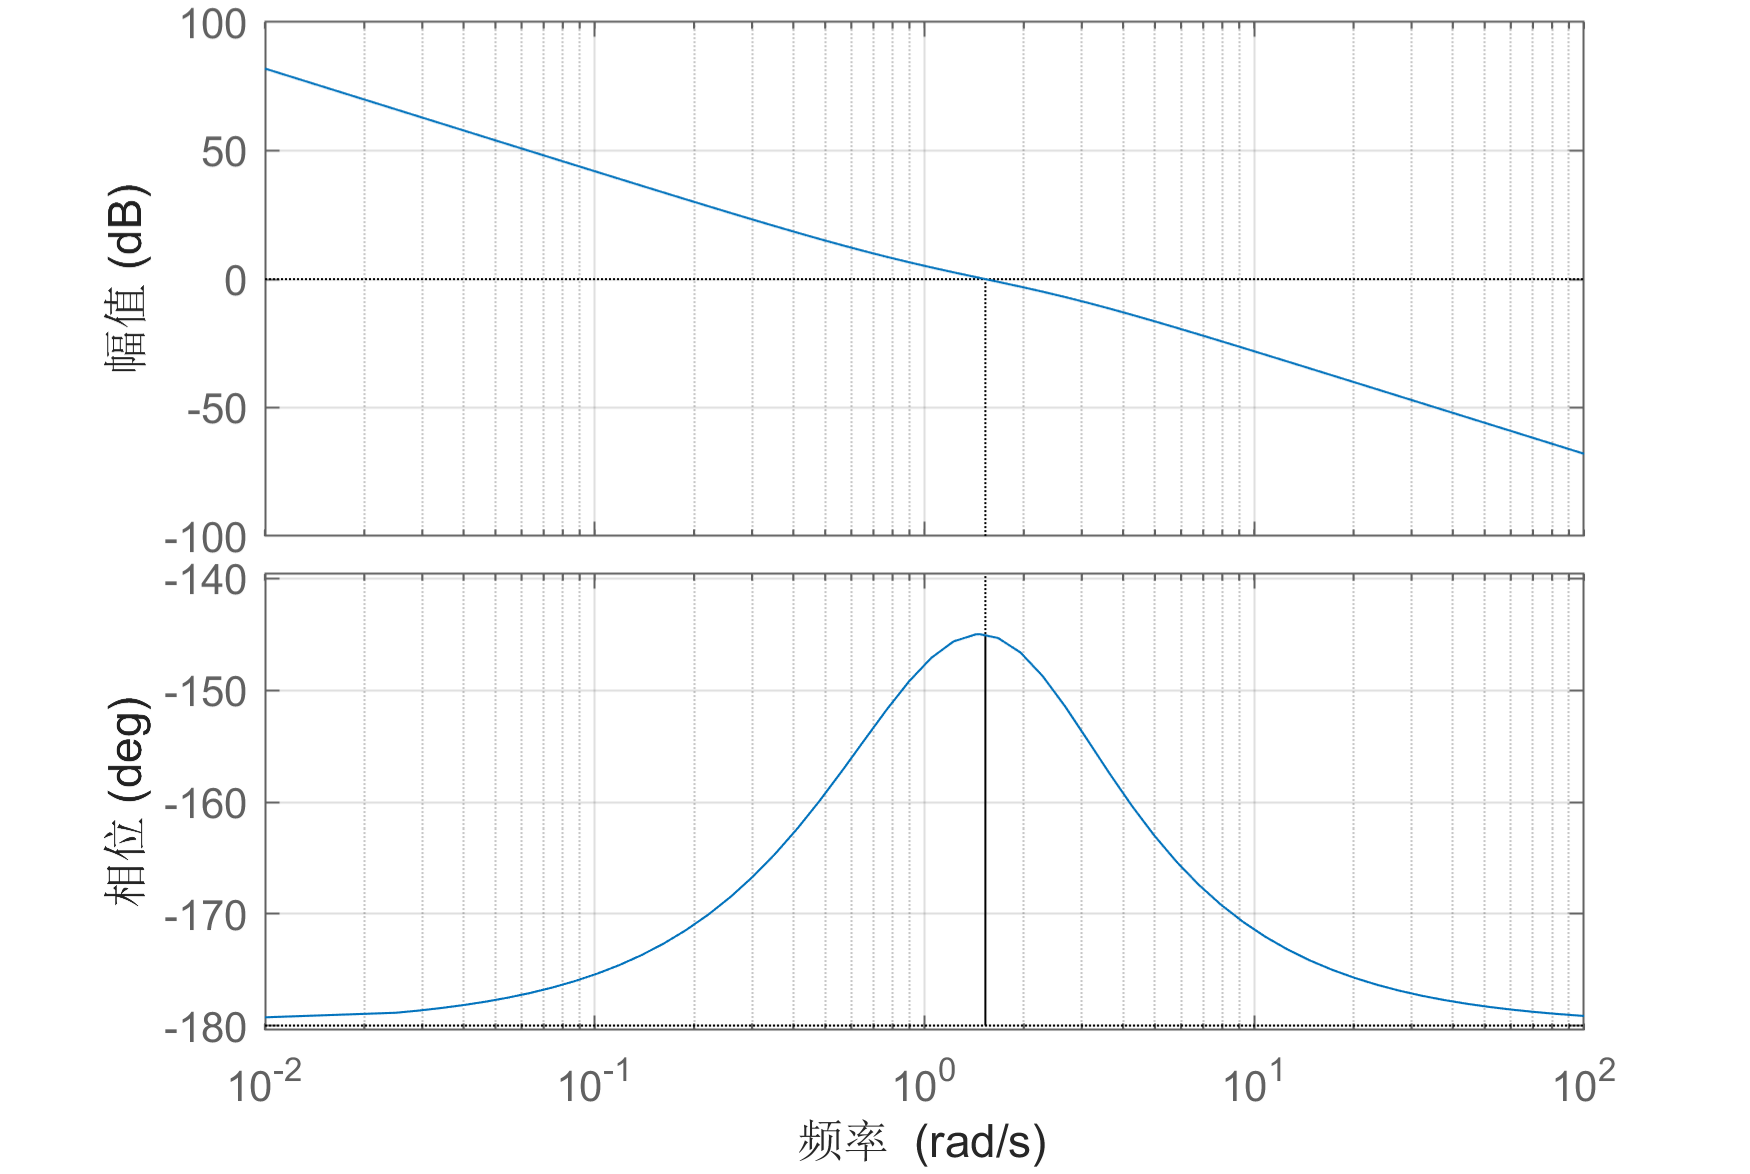
\includegraphics[width=0.8\textwidth]{Bode.png}
		% \framebox{\parbox{0.8\textwidth}{\centering \vspace{3cm} 插入Bode图 \vspace{3cm}}}
		\caption{系统开环 Bode 图}
		\label{fig:bode}
	\end{figure}
	
	根据 Bode 图及 MATLAB 仿真结果，我们可以获得系统的关键频域指标：
	
	\begin{itemize}
		\item \textbf{截止频率}：$\omega_c \approx 1.53 \, \text{rad/s}$。在此频率下，系统的开环幅值降为 0 dB。
		\item \textbf{相位裕度 }：$\gamma \approx 34.99^\circ$。这是在截止频率处，相位曲线距离 $-180^\circ$ 的差值。
	\end{itemize}
	
	\textbf{稳定性判别}：
	根据自动控制理论的稳定性判据，对于最小相位系统（或本例中的稳定开环极点系统），只要相位裕度 $\gamma > 0$，闭环系统即为稳定。
	从仿真结果来看，$\gamma = 34.99^\circ > 0$，且幅值裕度为无穷大（相位曲线在 0 dB 之前未穿越 $-180^\circ$ 线）。
	
	
	\subsection{闭环系统阶跃响应}
	
	本部分考察在不考虑前置滤波器（即 $G_p(s)=1$）时，上述闭环系统的单位阶跃响应性能。
	
	\subsubsection{闭环传递函数推导}
	
	系统为单位负反馈结构，闭环传递函数 $\Phi(s)$ 计算如下：
	\begin{equation}
		\begin{aligned}
			\Phi(s) 
			&= \frac{G_{\text{open}}(s)}{1 + G_{\text{open}}(s)} = \frac{\frac{4(s+1.25)^2}{s^2(s^2+4s+5)}}{1 + \frac{4(s+1.25)^2}{s^2(s^2+4s+5)}} \\
			&= \frac{4(s+1.25)^2}{s^2(s^2+4s+5) + 4(s+1.25)^2} \\
			&= \frac{4(s+1.25)^2}{(s^2+2s+2.5)^2}
		\end{aligned}
	\end{equation}
	
	令分母为零，可求得闭环极点为两对重根：
	\begin{equation}
		s_{1,2,3,4} = \frac{-2 \pm \sqrt{4 - 10}}{2} = -1 \pm j\sqrt{1.5} \approx -1 \pm j1.2247
	\end{equation}
	这一理论计算结果与 MATLAB 仿真输出的极点数据$-1.0000 \pm 1.2247i$一致。极点实部为负（$-1$），可验证系统的稳定性。
	
	\subsubsection{单位阶跃响应分析}
	
	进一步得到系统阶跃响应为： 
	\begin{equation}
		\Upsilon_1(s) = \frac{4(s+1.25)^2}{s(s^2+2s+2.5)^2}
	\end{equation}
	
	利用 MATLAB 求解系统对单位阶跃输入 $\theta_d(t)$ 的响应，所得曲线如图 \ref{fig:step} 所示。
	
	\begin{figure}[H]
		\centering
		% 注意：你需要确保工作目录下有名为 单位阶跃.png 的图片文件
		% 否则请注释掉下面一行，使用 framebox 替代
		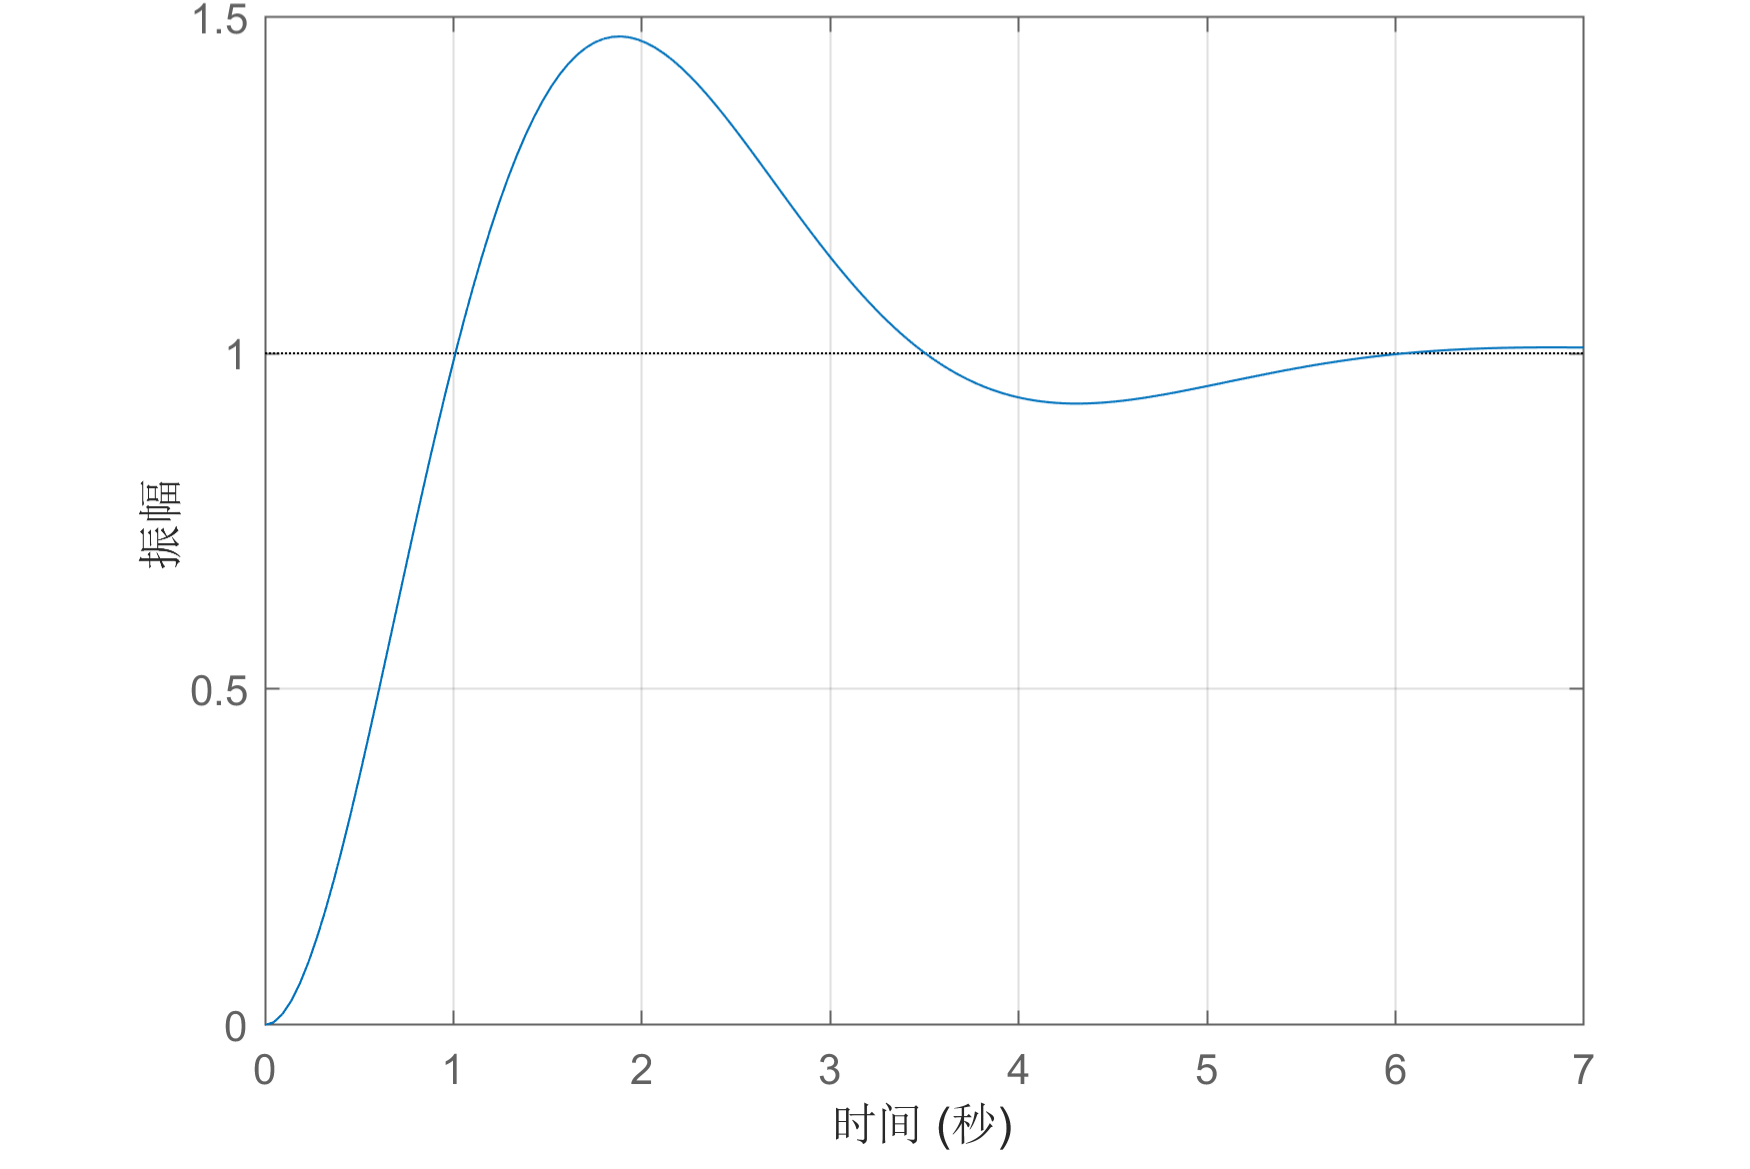
\includegraphics[width=0.5\textwidth]{单位阶跃.png}
		% \framebox{\parbox{0.8\textwidth}{\centering \vspace{3cm} 插入单位阶跃图 \vspace{3cm}}}
		\caption{闭环系统单位阶跃响应}
		\label{fig:step}
	\end{figure}
	
	根据仿真图像和数据，系统的动态性能指标如下：
	\begin{itemize}
		\item \textbf{超调量 (Overshoot)}：$\sigma \% \approx 47.17\%$。
		\item \textbf{调节时间 (Settling Time)}：$t_s \approx 5.52 \, \text{s}$（以 2\% 误差带计）。
		\item \textbf{稳态值}：系统最终收敛于 0.999365，有极小幅静态位置误差。
	\end{itemize}
	
	虽然系统是稳定的，但 47.17\% 的超调量过大，且调节时间较长。这说明系统的阻尼比偏小，动态响应表现出强烈的振荡特性，因此需要在系统里引入额外的环节进行矫正。
	
	\subsection{前置滤波器设计与系统改进}
	
	引入PID控制器的四阶闭环系统虽然稳定，但存在动态性能不佳的问题，特别是超调量高达 47.17\%。该问题主要源于闭环传递函数中存在一对距离虚轴较近的重零点 $s = -1.25$。在控制理论中，这类零点相当于引入微分作用，虽可加快系统响应，但也极易引发显著的超调。同时，原系统为一个四阶系统，其极点分布较为复杂，不利于性能的精确把控。
	
	为了解决上述问题，本部分将采用零极点对消的方法来构造前置滤波器 $G_p(s)$。我们的目标是通过前置滤波器抵消掉原闭环系统中的零点以及极点，并引入目标特征多项式，从而将复杂的四阶系统校正为一个标准的、性能优良的二阶系统。
	
	回顾第（4）问中推导出的闭环传递函数 $\Phi_{old}(s) = \frac{4(s+1.25)^2}{(s^2+2s+2.5)^2}$。 为了消除分子中 $(s+1.25)^2$ 带来的不利影响，我们在前置滤波器 $G_p(s)$ 的分母里引入 $(s+1.25)^2$项以对消零点。 同时，为简化原四阶结构，在 $G_p(s)$ 的分子中引入 $(s^2+2s+2.5)^2$ 项以对消原极点。 为实现理想的机械臂动态响应，我们目标是将系统校正为一个阻尼比 $\zeta = 0.707$ （工程最佳值）、自然频率 $\omega_n = 10$ rad/s（响应较快）的二阶系统。对应的目标特征多项式为 $s^2+2\zeta \omega_n s+\omega_n^2 = s^2+14.14s+100$。 于是构造前置滤波器如下：
	\begin{equation}
		G_p(s) = \frac{25(s^2 + 2s + 2.5)^2}{(s^2+14.14s+100)(s+1.25)^2}
	\end{equation}
	将此滤波器与原系统串联，得到新的闭环传函：
	\begin{equation}
		\Phi_{new}(s) = G_p(s) \cdot \Phi_{old}(s) = \frac{100}{s^2+14.14s+100}
	\end{equation}
	容易验证$\Phi_{new}(0) = 1$， 故系统对单位阶跃输入的稳态误差为零，稳态性能得以保持。此外，系统两个极点的实部都为$-7.07$，满足所有极点都在s平面的左半平面，因此系统稳定。
	
	此外， $G_p(s)$ 满足分子阶数 $\leq$ 分母阶数，是一个有理真分式， 且系数均为常实数， 因此具备物理可实现性。 同时， 该滤波器的两组极点 （二重实极点 $-1.25$ 、共轭复极点 $-7.07 + j7.07$）均在 $s$ 平面左半平面， 满足BIBO稳定， 输入有界时输出必然有界，符合滤波器工作的基本前提。 另外， $G_p(s)$ 幅频特性呈现低频衰减大、中频衰减小、高频衰减大的特性，是一个带通滤波器，核心通过频段为\(\omega \approx 10 \, \text{rad/s}\)，同时抑制低频（\(\omega \ll 1.225\)）和高频（\(\omega \gg 10\)）信号。
	
	于是进一步得到系统阶跃响应为： 
	\begin{equation}
		\Upsilon(s) = \frac{100}{s(s^2+14.14s+100)}
	\end{equation}
	
	对于校正后的二阶系统 $\Phi_{new}(s)$，自然频率 $\omega_n = 10$ 告诉我们系统响应较快； 阻尼比 $\zeta = 0.707$ 为工程最佳参数，这预示着系统不会产生过大的超调。
	
	\subsection{系统改进前后的对比分析}
	
	为了全面评估前置滤波器 $G_p(s)$ 的设计效果，我们将第（4）问中未校正系统的响应与第（5）问中校正后的系统响应进行了详细的对比。分析过程结合了时域仿真波形（如图 \ref{fig:compare} 所示）与具体的性能指标数据（如表 \ref{tab:comparison} 所示）。
	
	\subsubsection{仿真波形对比}
	
	首先，我们将改进前后的单位阶跃响应曲线绘制在同一坐标系下进行比较。
	
	\begin{figure}[H]
		\centering
		
\includegraphics[width=0.8\textwidth]{6.png}
		\caption{引入前置滤波器前后的系统阶跃响应对比}
		\label{fig:compare}
	\end{figure}
	
	从图 \ref{fig:compare} 中可以清晰地观察到，未校正的系统（红色）在达到稳态前经历了大幅的超调且进入2\%误差带耗时较长；而校正后的系统（蓝色）响应曲线变得非常平滑，小幅超调，快速响应。
	
	\subsubsection{性能指标量化对比}

为了更严谨地说明问题，我们将两个系统的关键性能指标汇总于下表：

\begin{table}[H]
	\centering
	\caption{系统改进前后性能指标对比表}
	\label{tab:comparison}
	\renewcommand{\arraystretch}{1.2} % 调整行高
	\begin{tabular}{ccc}
		\toprule
		\textbf{性能指标} & \textbf{改进前（无 $G_p$）} & \textbf{改进后（有 $G_p$）} \\
		\midrule
		稳态值 & 0.999365 & 1.000000 \\
		峰值 & 1.471725 & 1.043255 \\
		超调量 ($\sigma\%$) & 47.17\% & 4.33\% \\
		调节时间 ($t_s$, 2\%误差带) & 5.52 s & 0.597 s \\
		IAE (积分绝对误差) & 1.403 & 0.161 \\
		ISE (积分平方误差) & 0.703 & 0.106 \\
		\bottomrule
	\end{tabular}
\end{table}

结合图表数据，我们可以得知：

\begin{itemize}
	\item \textbf{超调量的显著抑制}：这是本次设计最核心的改进点。原系统的超调量高达 47.17\%，这在实际机械手控制中是不可接受的，因为它意味着机械臂会大幅冲过目标位置，极易造成碰撞或设备损坏。引入 $G_p(s)$ 后，通过零极点对消消除了微分效应，将超调量大幅降低至 4.33\%，使得系统运行更加平稳柔和。
	
	\item \textbf{调节速度的提升}：原系统花费了 5.52 秒才稳定在误差范围内，而改进后的系统得益于工程最佳阻尼比（$\zeta = 0.707$）的配置，它能够更果断地收敛，将调节时间缩短至 0.597 秒，这意味着机械手能更快地完成定位任务。
	
	\item \textbf{模型的简化与可控性}：从理论层面看，前置滤波器将原本复杂的 4 阶系统简化为了标准的 2 阶系统。这种“模型降阶”不仅让响应曲线更符合预期，也降低了后续控制器调试的难度。
\end{itemize}

通过设计前置滤波器 $G_p(s)$ 来调整系统特性，我们取得了系统稳定性和快速性的巨大提升。这一设计成功解决了原系统动态性能差的问题，完全达到了预期的控制目标。

\section{精馏过程控制系统}
\subsection{精馏过程工艺结构及操作机理}
精馏是化工分离中应用最为广泛的技术之一，其核心原理在于利用混合物中各组分挥发度（或沸点）的差异，通过多次部分汽化与部分冷凝的过程实现高效分离。挥发度较大的轻组分沸点较低，易于汽化；而挥发度较小的重组分沸点较高，难以汽化。操作中，通过加热使混合物部分汽化，产生蒸汽和液体两相，其中蒸汽富含轻组分，液体则富含重组分。随后，蒸汽与液体在塔内进行多级、逆向的接触，经历反复的部分汽化与部分冷凝，从而在塔顶获得高纯度的轻组分产品，在塔底获得高纯度的重组分产品。

精馏塔的工艺结构通常包括塔体、进料板、冷凝器、再沸器和回流罐等关键部分。塔体多为直立圆筒形设备，内部装有塔板或填料，以提供气液两相充分接触的传质界面。塔板（如筛板、浮阀塔板）上维持一定液层，蒸汽鼓泡通过液层实现传质；填料（如规整填料）则依靠其高比表面积促进相际接触。进料板是原料加入的位置，以此将塔划分为精馏段和提馏段：精馏段位于进料板之上，其主要作用是通过冷凝下降液体中的重组分，使上升蒸汽中轻组分浓度不断升高；提馏段位于进料板之下，其作用是通过汽化上升蒸汽中的轻组分，使下降液体中重组分浓度增加。冷凝器置于塔顶，将上升蒸汽冷凝为液体，若为全凝器，则冷凝液一部分作为产品采出，另一部分作为回流返回塔内；再沸器位于塔底，提供热源使塔底液体部分汽化，产生上升蒸汽。回流罐则用于稳定回流量，维持塔内物料平衡。这一结构设计支持连续化操作，并通过调节进料位置和塔内构件优化分离效率。

精馏过程的实现依赖于物料平衡、气液平衡与传质、热量平衡与传热以及回流作用等多重操作机理的协同。物料平衡是基础，即总进料量等于塔顶和塔底采出量之和，各组分也需满足物料平衡，否则将引起组成波动。气液平衡与传质发生在每一块塔板或填料表面：上升蒸汽与下降液体逆流接触，轻组分从液相向气相转移，重组分从气相向液相转移，通过多级平衡接触，蒸汽中轻组分浓度逐板升高，液体中重组分浓度逐板增加，从而实现分离。热量平衡由再沸器输入热量和冷凝器输出热量所控制，决定了塔内的温度分布——塔顶温度较低，对应于轻组分的沸点；塔底温度较高，对应于重组分的沸点，这一温度梯度反映了组成分布，是精馏控制的关键指标。回流则是实现高纯度分离的必要条件，回流比（定义为回流量与采出量之比）直接影响分离效果和能耗：提高回流比可增强分离效果，但同时也增加了能量消耗，故需在保证产品质量的前提下进行优化选择。这些机理共同作用，确保了精馏过程的稳定与高效。

以进料板为界，精馏塔分为精馏段与提馏段，两段功能各有侧重。精馏段的主要功能是提升塔顶轻组分产品的纯度，通过上升蒸汽与回流液体的逆流接触，重组分被冷凝下来，轻组分则不断汽化并富集于塔顶。提馏段的主要任务是从下降液体中剥离轻组分，从而提高塔底重组分的纯度，该段通过再沸器产生的热蒸汽与下流液体接触，使轻组分被汽提并随蒸汽上升，重组分则继续向下流动。精馏段内气液两相流量相对稳定，回流比是影响其分离效率的关键参数；提馏段内液相流量较大，再沸器的供热能力对其分离效果具有显著影响。完整的精馏塔须同时包含精馏段与提馏段，方可实现从塔顶和塔底连续获取高纯度产品。

回流在精馏过程中扮演着不可或缺的角色，它为下降液体提供了来源，并与上升蒸汽进行逆流接触。回流比作为一个核心操作参数，其大小直接关系到分离效率与能耗：回流比增大，分离效果提高，但再沸器加热量与冷凝器冷却量也随之增加，导致操作成本上升。因此，在实际操作中需在满足产品质量要求的前提下，寻求回流比的最优值以实现节能。回流比的调控可通过调节回流量或采出量来实现，同时，塔内温度与压力的变化也会对回流条件产生影响，进料流量的波动同样可能要求调整回流比以维持分离效果。由此可见，回流作用的有效调控是精馏过程稳定运行与优化操作的关键环节。

\subsection{精馏过程关键工艺参数及主要扰动分析与阐述}

精馏过程的经济性与操作稳定性在很大程度上取决于对关键工艺参数的精确控制以及对主要扰动的有效抑制。该过程的稳态运行由物料平衡、能量平衡与气液平衡共同决定，工业装置中则通过一系列相互关联的控制系统来维持这一动态平衡。在精馏塔的多变量控制体系中，塔顶与塔底温度的控制尤为关键，因其直接关联最终产品的纯度。塔顶温度控制系统常采用串级控制策略，以塔顶温度作为主被控变量，回流流量作为副被控变量兼操纵变量。该方案能有效克服进料组成变化、冷却剂压力波动及塔压波动等干扰。其控制机理在于，当干扰导致塔顶温度偏离设定值时，主调节器通过改变副回路的设定值，由副调节器快速调整回流量，进而改变塔内气液平衡状态，及时纠正温度偏差，从而保障轻组分产品的质量。类似地，塔底温度控制系统也采用串级结构，以塔底温度为主被控变量，加热蒸汽流量为副被控变量。此设计能够有效抑制蒸汽总管压力波动和进料焓值变化对塔底重组分纯度的影响，通过调节再沸器的热负荷来稳定提馏段的操作。

塔压是精馏过程的一个基本参数，其稳定性至关重要。塔压波动会直接影响塔内温度分布和各组分的相对挥发度，进而对分离效率产生显著影响。塔压控制系统通常以塔顶压力为被控变量，通过调节冷凝器的冷却剂流量来改变系统的热移除速率，从而维持压力恒定。该单回路控制方案需要应对进料气化率变化、再沸器加热量波动等干扰，其稳定运行是其他温度、液位控制回路得以正常工作的前提。

液位控制是维持塔内物料平衡、保证连续平稳操作的关键。回流罐（或冷凝罐）液位控制系统通过调节塔顶产品的采出量来维持液位稳定，主要克服因冷凝器冷凝速率变化和回流量调整所带来的干扰。塔底液位控制系统则通过调节塔底产品的采出量来应对下流液量和蒸发量的波动。这两个单回路控制系统共同确保了塔内持液量的稳定，为连续的分离过程提供了必要的物料平衡基础。

此外，进料流量作为过程的输入变量，其稳定性对整个精馏塔的平稳运行具有基础性作用。进料流量控制系统通常采用单回路定值控制，通过调整进料阀的开度来克服前序工序供料压力波动等干扰，使进料流量保持恒定，从而为精馏塔建立稳定的操作条件。

综上所述，精馏过程的工艺控制是一个多变量、强耦合的复杂系统。关键工艺参数如温度、压力、液位及回流比等并非孤立存在，而是通过上述控制回路相互关联，构成一个有机整体。采用如串级控制的先进策略，通过引入中间变量增强了系统对抗主要扰动的能力。参数优化与扰动管理的核心目标，在于借助系统化的自动控制手段，将精馏过程稳定在最优操作点附近，最终实现分离效率、产品质量与能源消耗之间的最佳平衡。

\subsection{控制系统原理图分析}

在精馏塔的运行过程中，塔底产品的纯度是一个极为关键的质量指标。通常情况下，我们并不直接在线测量成分，而是选取与成分有对应关系的塔底温度作为被控变量。

在分析塔底温度的控制方案时，我们需要考虑到工业现场存在多种干扰因素。其中，加热蒸汽压力的波动是最常见且影响最大的干扰。如果采用简单的单回路控制，当蒸汽压力波动引起流量变化时，必须等到塔底温度发生改变后，控制器才会动作。由于温度对象具有较大的热惯性，这种滞后的调节往往无法满足高质量的生产要求。

因此，该系统采用的是塔底温度与加热蒸汽流量的串级控制方案。系统的核心在于构建了两个闭环回路。副回路直接检测并控制进入再沸器的蒸汽流量，主回路则负责检测塔底温度并调整副回路的设定值。

如图 \ref{fig:cascade_principle} 所示，这种结构的优势在于它能将干扰“分而治之”。凡是引起蒸汽流量波动的干扰，如管网压力变化，都会被副回路在第一时间发现并消除，不再影响主回路的温度。而对于进料成分变化等其他干扰，则由主回路进行调节。这种主副配合的模式，极大地提高了系统对干扰的抑制能力，从而保证了塔底温度的平稳。

\begin{figure}[H]
	\centering
	% 此处使用您指定的塔底温度控制系统图作为原理示意
	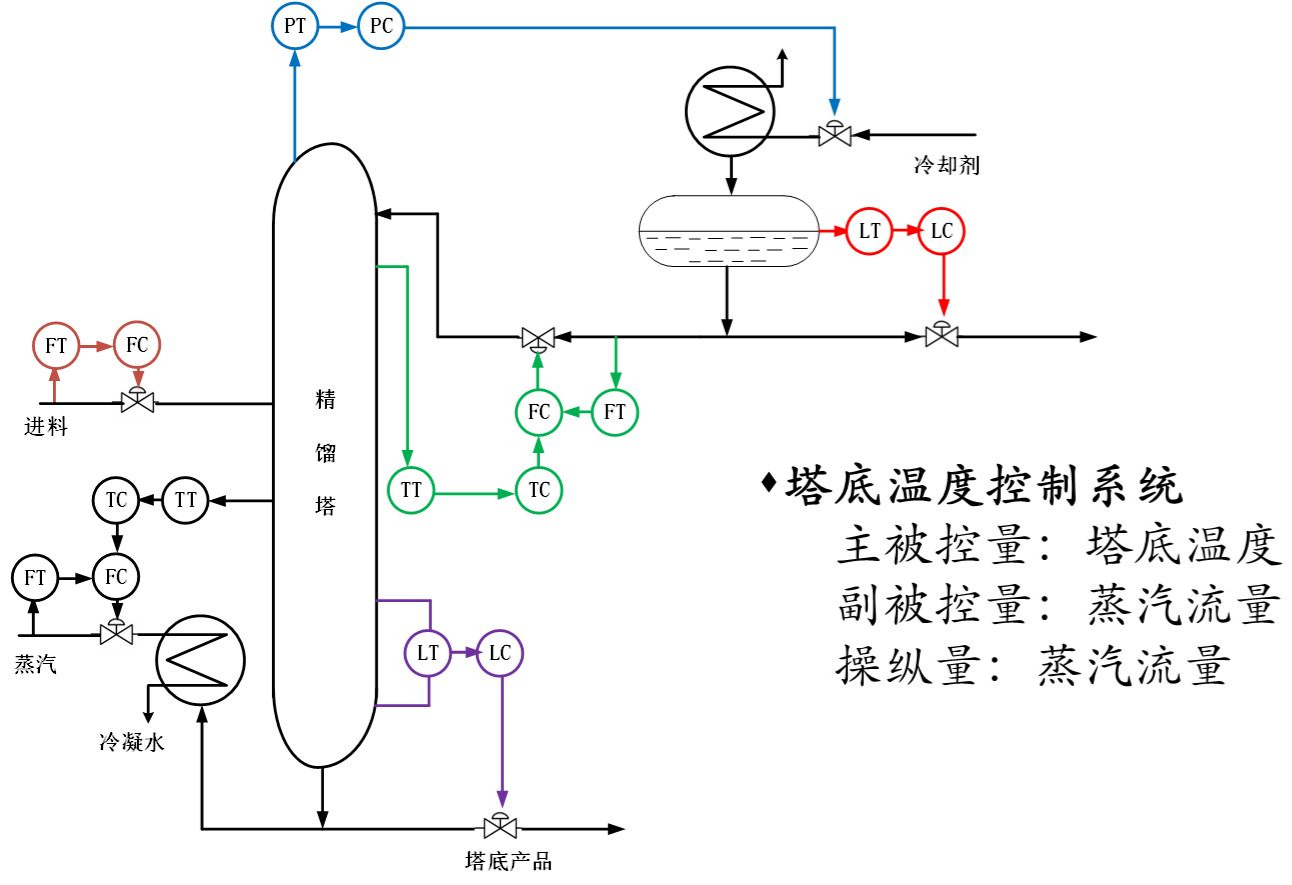
\includegraphics[width=0.8\textwidth]{塔底温度.png}
	\caption{塔底温度-蒸汽流量串级控制系统原理图}
	\label{fig:cascade_principle}
\end{figure}

\subsection{控制系统方框图与详细分析}

\subsubsection{精馏塔总体控制方案分析}

精馏塔是一个复杂的化工设备，其内部的气液相平衡依赖于多个工艺参数的协同稳定。根据课程设计任务书给定的对象模型及工艺要求，该精馏塔的控制系统被划分为六个独立的子系统。这些子系统各司其职，共同维持物料平衡和能量平衡。

我们可以从上至下对这六个控制回路进行梳理：

首先是塔顶区域。为了保证塔顶轻组分的纯度，系统设置了塔顶温度控制回路（图 \ref{fig:loop_1}）。它通过调节回流阀的开度来改变回流量，从而控制精馏段的温度。与之配合的是冷凝罐液位控制回路（图 \ref{fig:loop_2}），它通过调节产品的采出量来维持回流系统的物料平衡。

其次是压力环境。塔压的稳定是分离过程进行的基础。塔压控制回路（图 \ref{fig:loop_3}）通过调节冷凝器中冷却剂的流量，改变移热速率，从而克服干扰维持塔压恒定。

接着是核心的提馏段。为了确保塔底重组分的质量，系统配置了塔底温度串级控制回路（图 \ref{fig:loop_4}）。这也是我们重点分析的对象，它通过精细调节加热蒸汽量来控制釜温。同时，为了防止再沸器出现干烧或溢出，设有塔底液位控制回路（图 \ref{fig:loop_5}），利用塔底产品的采出量来平衡液位。

最后是进料源头。进料流量控制回路（图 \ref{fig:loop_6}）位于工艺最前端，它通过定值控制消除上游的压力波动，为后续的分离过程提供稳定的负荷。
\subsubsection{塔底温度串级系统的详细分析}

在上述六个系统中，塔底温度串级控制系统最为复杂也最为关键。要理解该系统的工作逻辑，我们需要对其中的调节阀选择和控制器作用方向进行深入分析。

首先分析调节阀的气开与气关选择。这一选择主要依据“故障安全”原则。在该系统中，调节阀控制的是进入再沸器的加热蒸汽。我们设想最坏的情况，如果控制信号中断或者气源发生故障，阀门将回复到自然状态。此时，为了防止再沸器持续加热导致塔内超压、物料分解甚至发生爆炸事故，阀门必须自动关闭以切断热源。因此，该蒸汽调节阀应选择气开式。即有气压信号时阀门打开，无信号时自动关闭。

确定了调节阀为气开式后，我们就可以分析控制器的正反作用方向。控制系统的基本原则是构成负反馈，即控制器的作用方向应能抵消被控变量的偏差。

对于副回路（流量环）：假设蒸汽流量因干扰而增加，为了将其拉回设定值，需要关小阀门。由于阀门是气开式，关小阀门意味着减小控制器的输出信号。即测量值增加导致控制器输出减小，输入与输出变化方向相反。因此，副控制器（FC）应选择反作用。

对于主回路（温度环）：假设塔底温度升高，说明热量输入过多。为了降低温度，主控制器需要减少对蒸汽流量的需求，也就是减小给副回路的流量设定值。同样地，测量值温度的增加要求控制器输出减小，输入与输出变化方向相反。因此，主控制器（TC）也应选择反作用。

综上所述，该串级系统通过气开式调节阀与两个反作用控制器的配合，构建了逻辑严密的负反馈调节机制。

\begin{figure}[H]
	\centering
	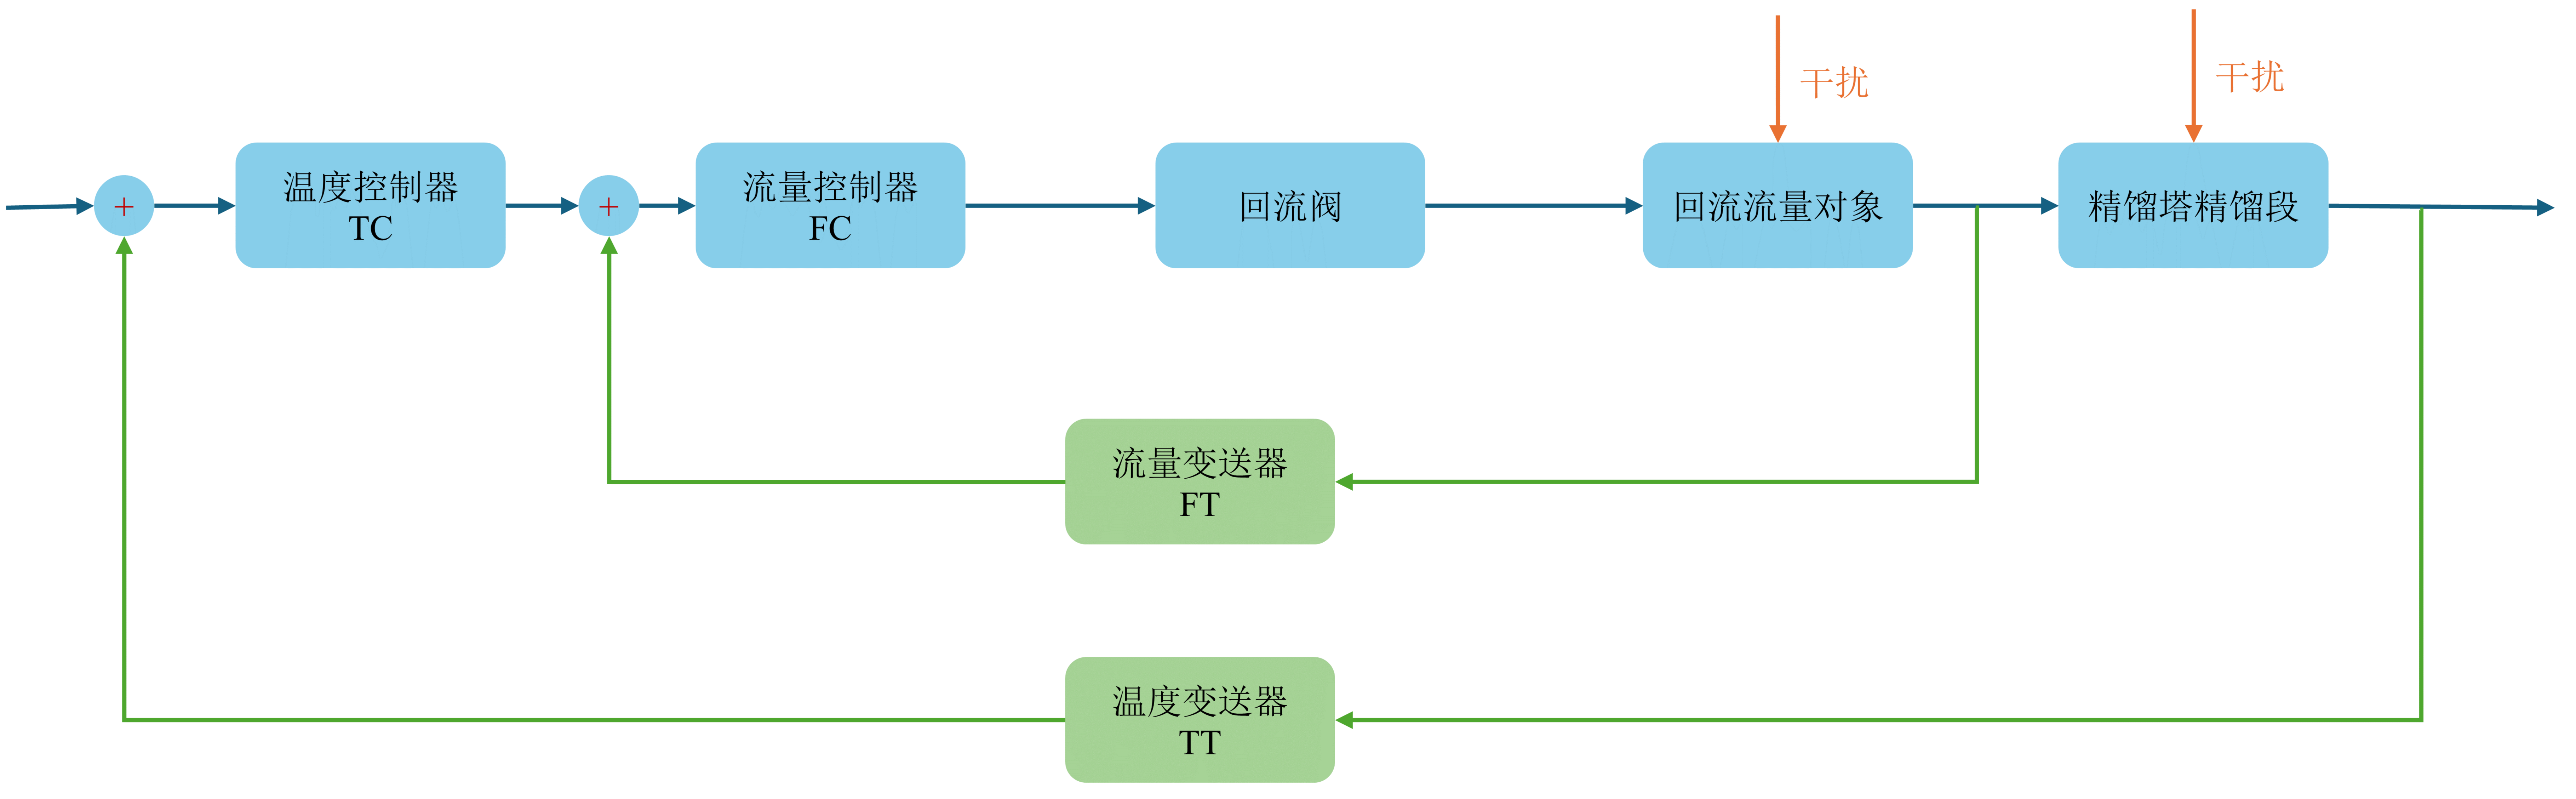
\includegraphics[width=0.8\linewidth]{1塔顶温度控制系统.png}
	\caption{塔顶温度控制系统方框图}
	\label{fig:loop_1}
\end{figure}

\begin{figure}[H]
	\centering
	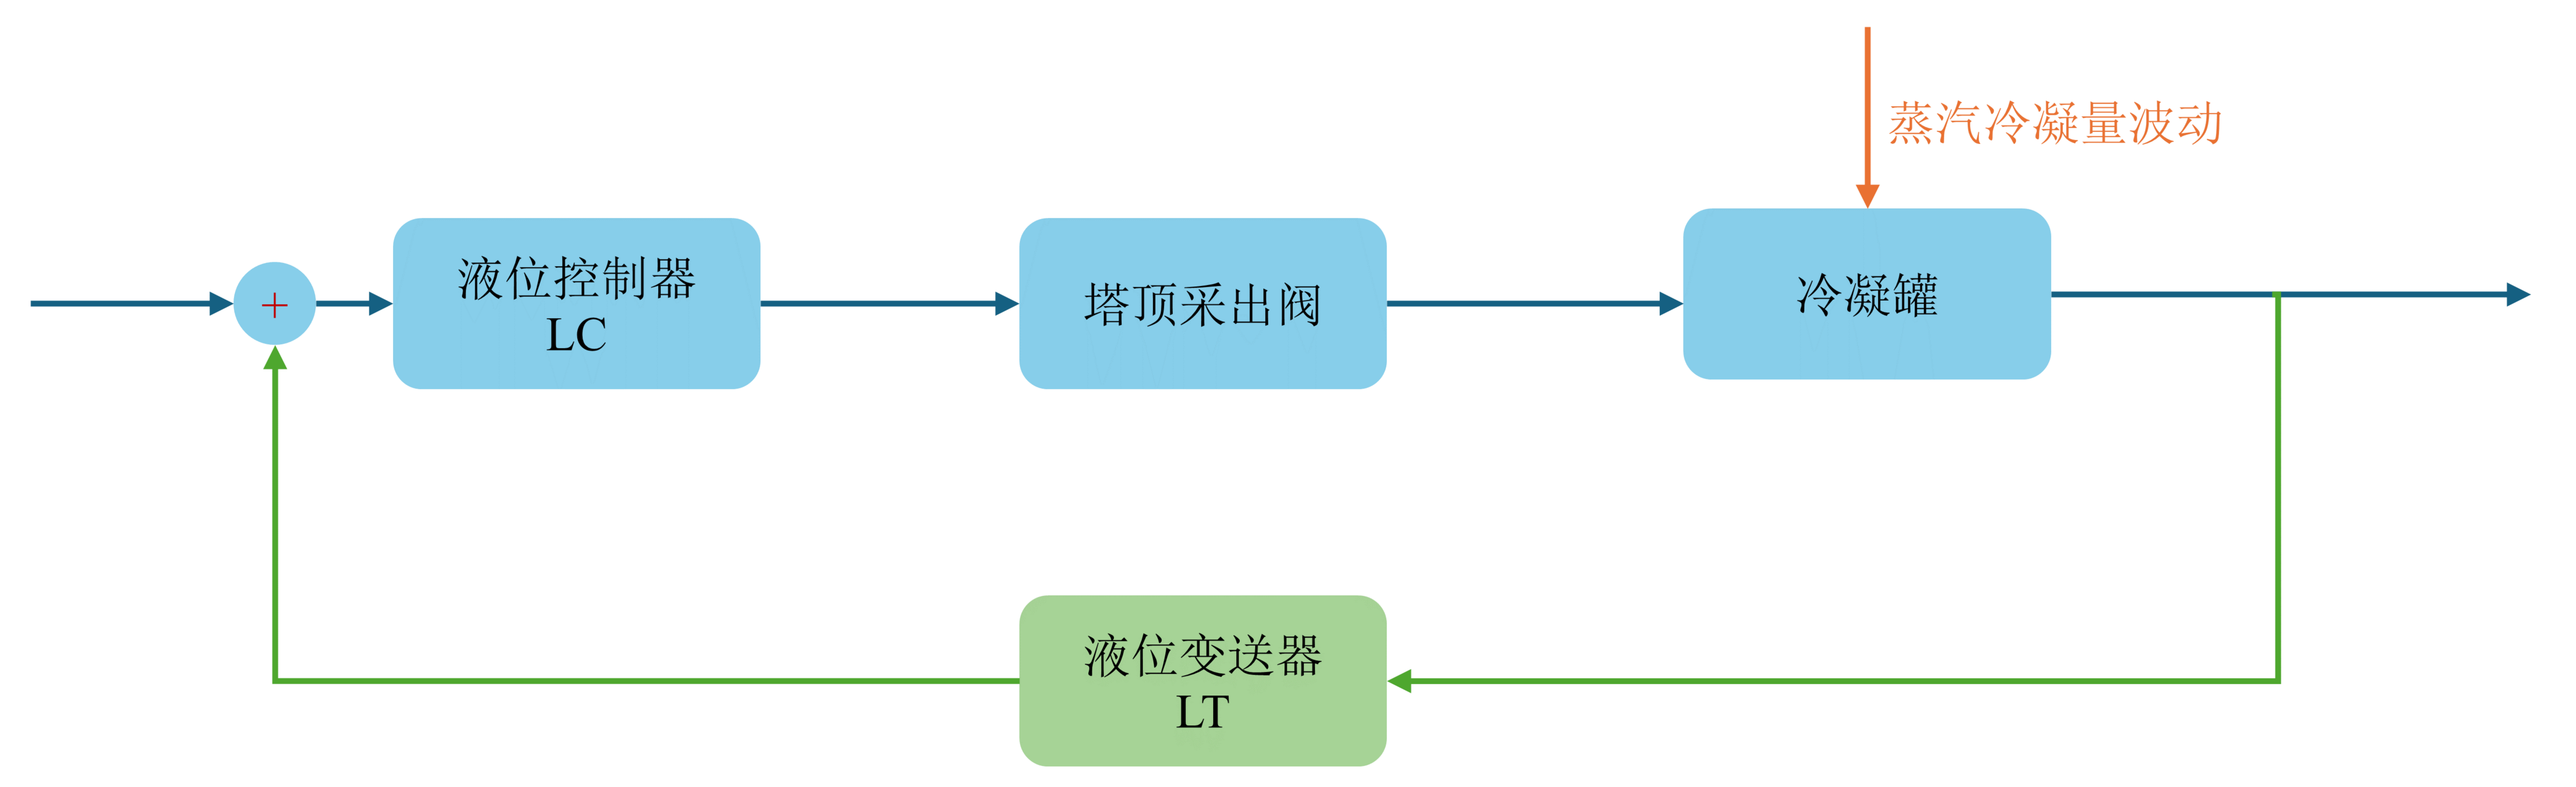
\includegraphics[width=0.8\linewidth]{2冷凝罐液位控制系统.png}
	\caption{冷凝罐液位控制系统方框图}
	\label{fig:loop_2}
\end{figure}

\begin{figure}[H]
	\centering
	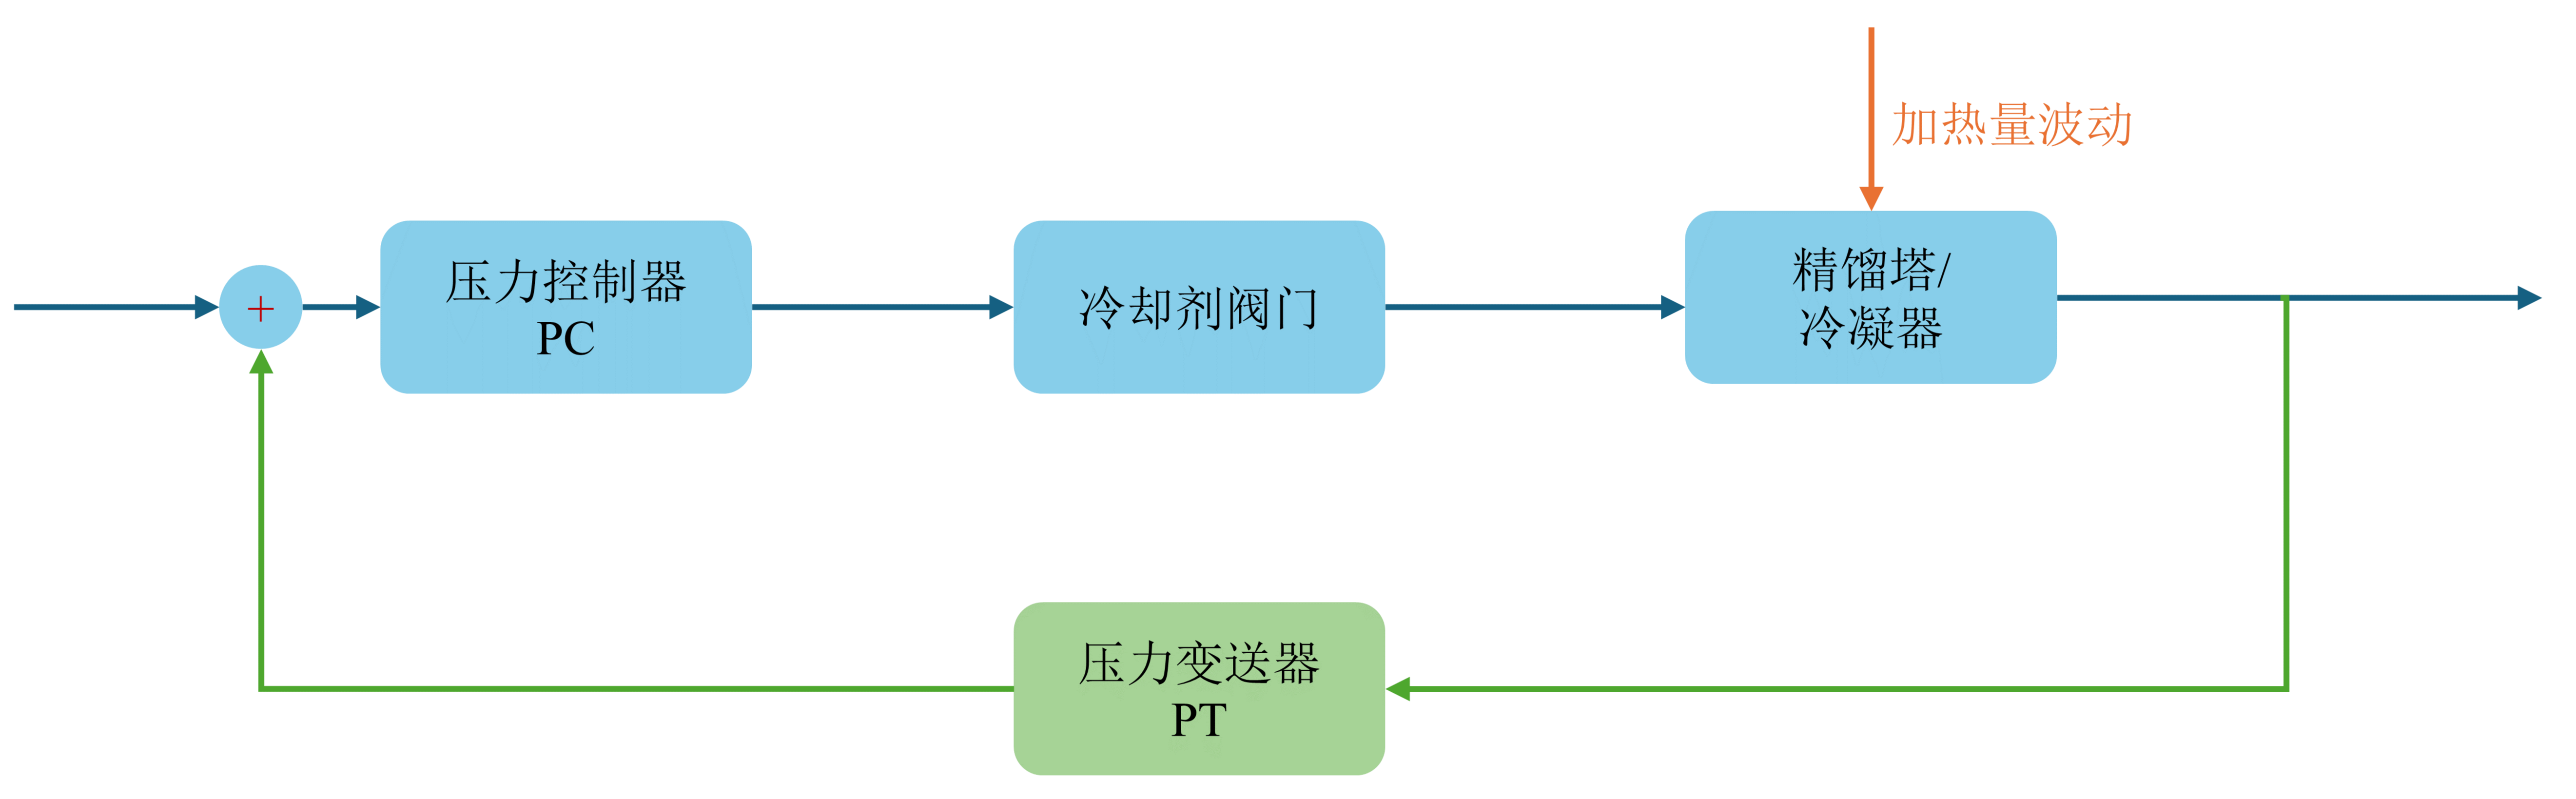
\includegraphics[width=0.8\linewidth]{3塔压控制控制系统.png}
	\caption{塔压控制系统方框图}
	\label{fig:loop_3}
\end{figure}

\begin{figure}[H]
	\centering
	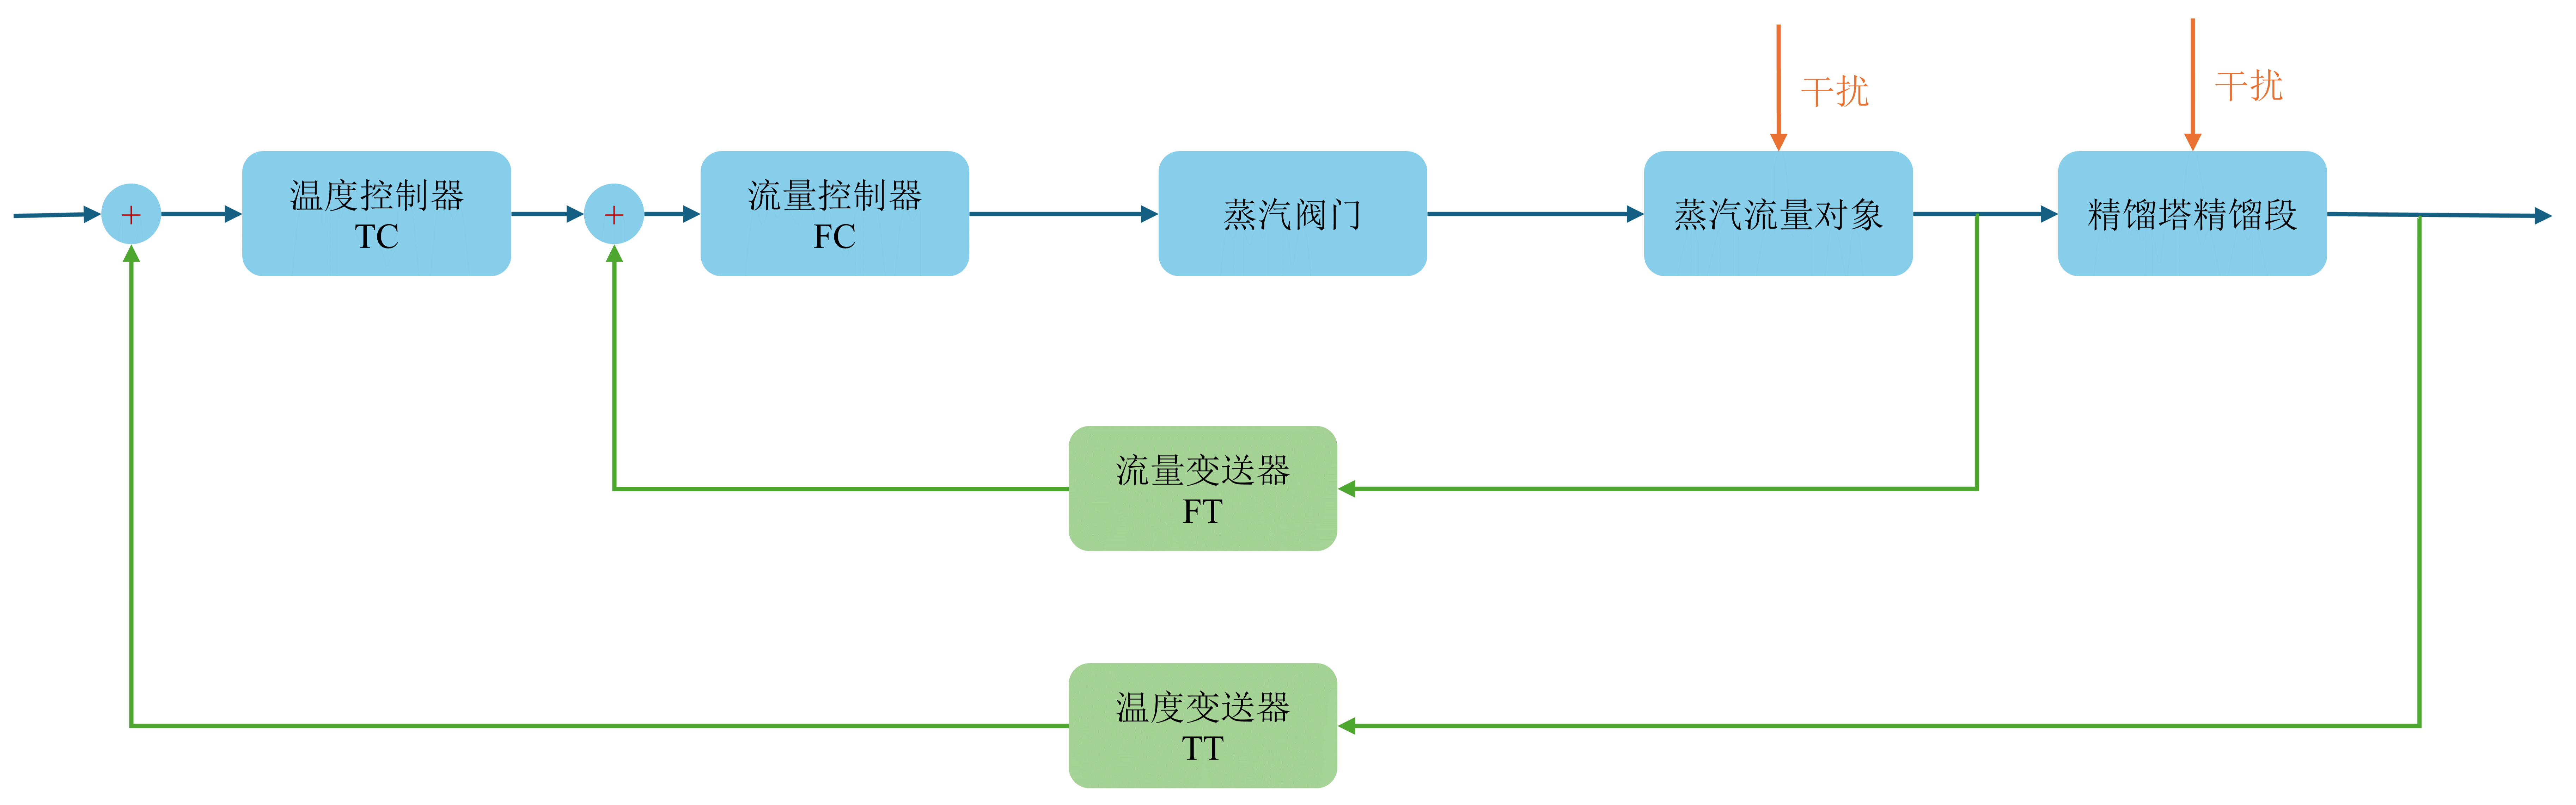
\includegraphics[width=0.8\linewidth]{4塔底温度控制系统.png}
	\caption{塔底温度控制系统方框图}
	\label{fig:loop_4}
\end{figure}

\begin{figure}[H]
	\centering
	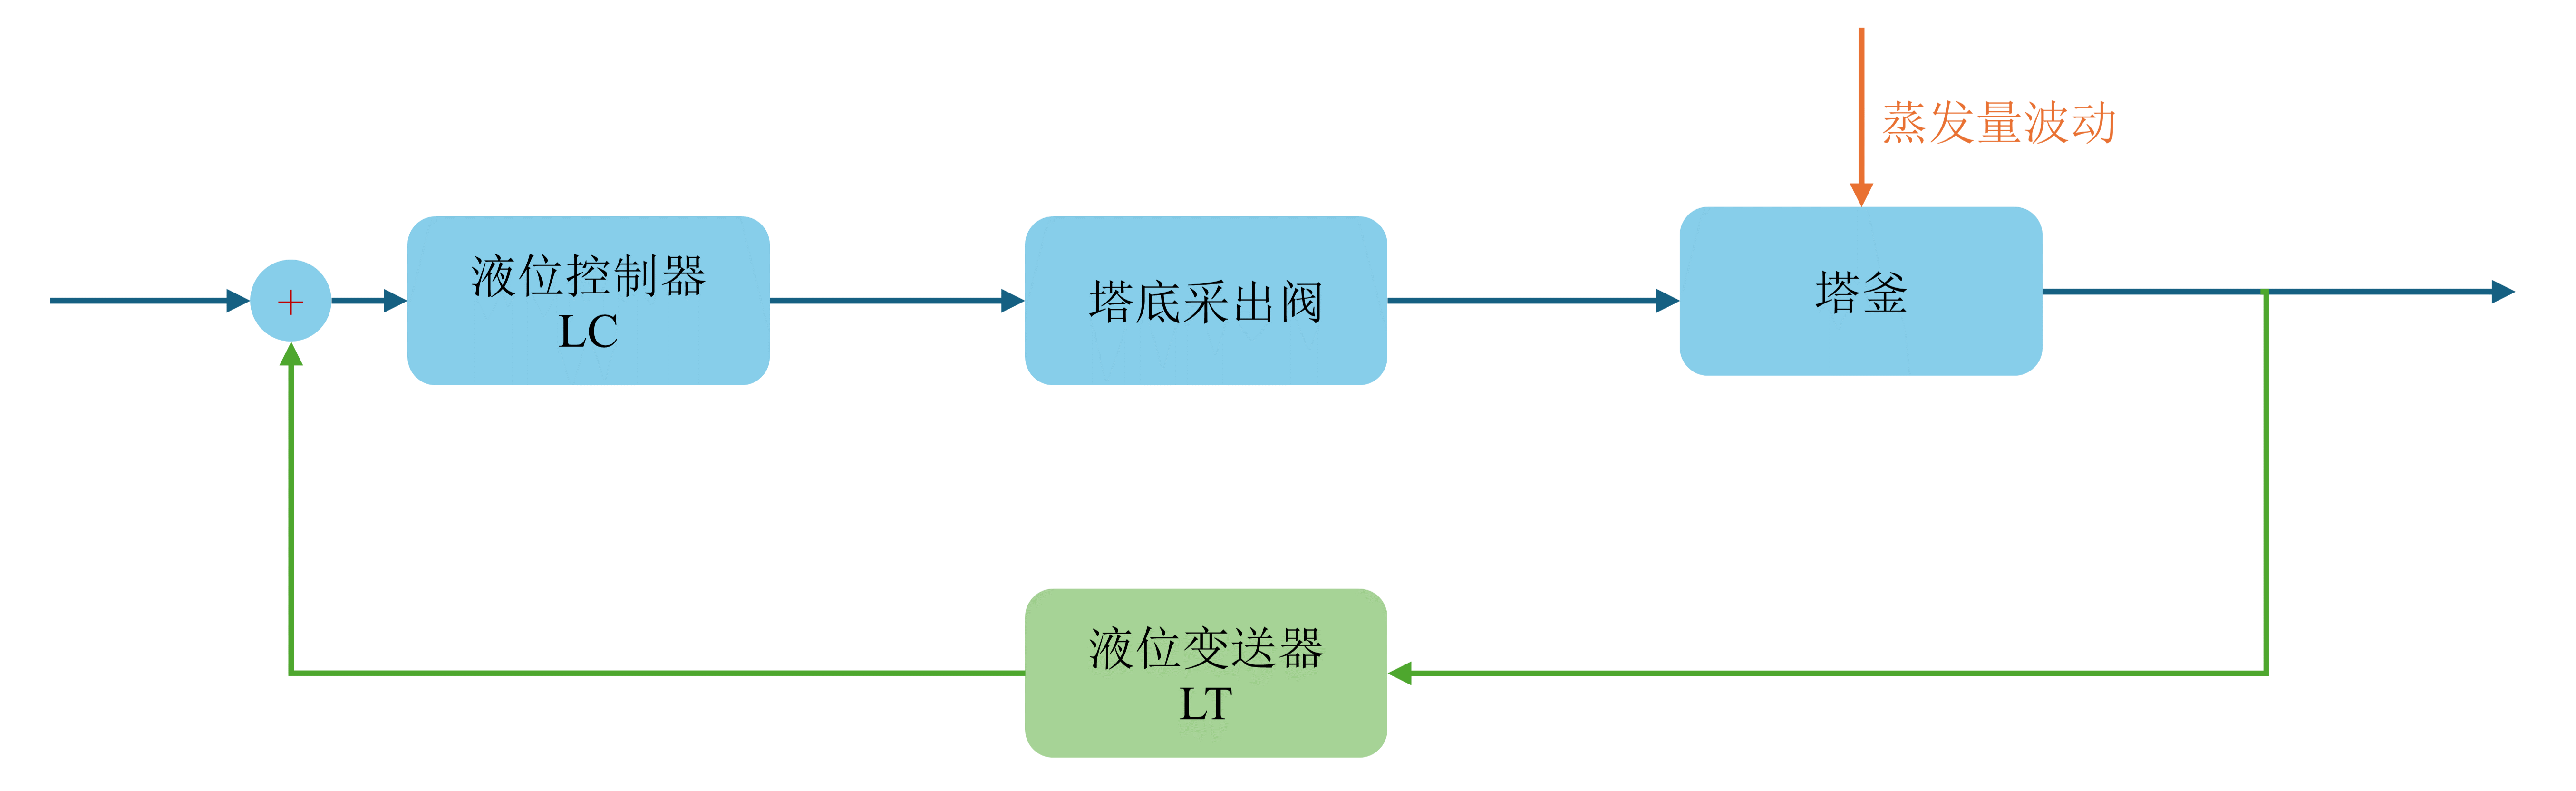
\includegraphics[width=0.8\linewidth]{5塔底液位控制系统.png}
	\caption{塔底液位控制系统方框图}
	\label{fig:loop_5}
\end{figure}

\begin{figure}[H]
	\centering
	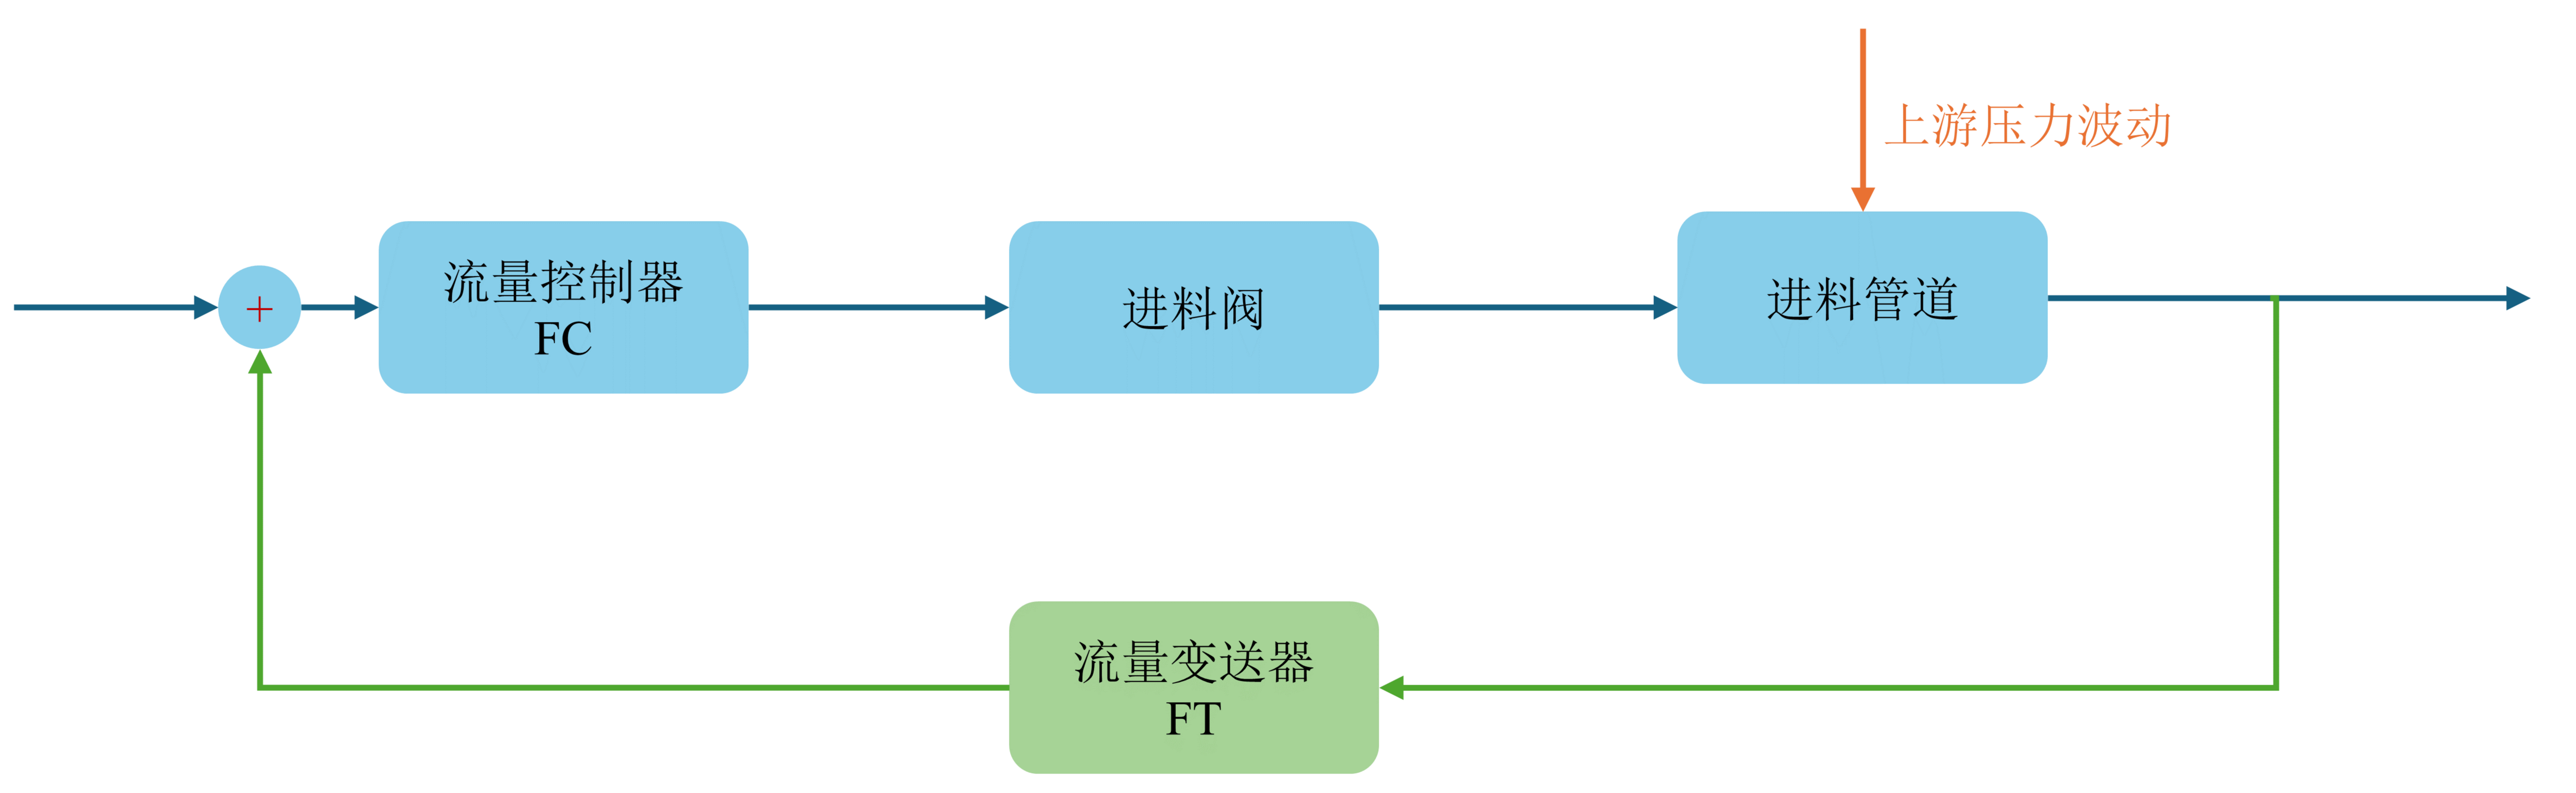
\includegraphics[width=0.8\linewidth]{6进料流量控制系统.png}
	\caption{进料流量控制系统方框图}
	\label{fig:loop_6}
\end{figure}




\subsubsection{塔底温度串级控制系统的详细设计}
在上述六个子系统中，我们重点对图 \ref{fig:loop_4} 所示的塔底温度串级控制系统进行深入设计。为了使该控制方案在工程实际上切实可行，必须正确选择执行机构的作用方式以及控制器的正反作用方向。

调节阀的气开/气关形式选择遵循“生产安全第一”的原则。在本系统中，执行机构调节的是进入再沸器的加热蒸汽流量。考虑到工业现场可能出现的气源故障或控制信号中断等极端情况，为了防止在失控状态下再沸器持续加热，导致塔内压力急剧升高、物料分解变质甚至引发爆炸事故，调节阀必须具备故障自动切断热源的功能。因此，该蒸汽调节阀应选用气开式，即只有在接收到气压信号时阀门才打开，无信号时自动回复到全关状态。

基于调节阀的气开特性，我们需要进一步推导主、副控制器的正反作用，以确保各回路均构成负反馈。首先分析副回路（流量环）：当测量到的蒸汽流量增加时，为了将流量拉回设定值，控制器需要减小阀门开度；对于气开阀而言，减小开度意味着减小控制信号输出。即测量值增加导致输出减小，因此副控制器应选择反作用。

接着分析主回路（温度环）：当塔底温度升高超过设定值时，意味着输入热量过多，主控制器应降低对蒸汽流量的需求，即减小副回路的设定值。同样地，测量值（温度）的增加要求控制器输出（流量设定值）减小，因此主控制器也应选择反作用。这种双反作用的配置，配合气开式调节阀，构成了逻辑严密的串级负反馈系统。

\subsection{仿真分析与参数整定}

\subsubsection{仿真环境构建与模型参数说明}
为了全面验证本文所设计的塔底温度串级控制策略的有效性与鲁棒性，我们依据课程设计任务书中所提供的化工过程数学模型，搭建了数字化仿真实验平台。该平台的核心任务是模拟精馏塔提馏段在真实工况下的动态响应，并以此为基础进行控制器的参数寻优。

仿真模型主要包含两个核心环节。首先是副回路对象，即加热蒸汽流量通道。根据工艺特性分析，调节阀开度对蒸汽流量的影响响应较快，因此将其近似为一个一阶惯性环节，其传递函数为 $W_3(s) = \frac{1}{2s+1}$。该模型反映了流量随阀门动作的快速跟随特性，是串级控制中能够快速抑制压力干扰的基础。其次是主回路对象，即塔底温度通道。由于热容量大且传热过程复杂，蒸汽流量对塔底温度的影响表现出显著的大惯性和大滞后特征，故将其建模为二阶滞后环节，其传递函数为 $W_4(s) = \frac{2}{(120s+1)(130s+1)}$。这两个差异巨大的时间常数（2s 对比 120s/130s）构成了典型的串级控制对象特征，要求控制器设计必须兼顾快速性与稳定性。

\subsubsection{基于网格搜索的参数整定策略}
针对串级控制系统中主、副控制器参数耦合难以整定的问题，本次设计采用了一种基于性能指标优化的智能化网格搜索算法（Grid Search）。该算法能够在预设的参数空间内进行遍历搜索，以寻找使系统综合性能最优的参数组合。整定过程严格遵循“先内环、后外环”的工程原则，具体实施步骤如下：

第一阶段主要针对响应较快的副回路（流量环）进行整定。考虑到流量环的主要任务是快速消除内环干扰并随动于主控制器的输出，且在尝试加入D控制效果并不好之后，我们选择了PI控制器。在搜索范围内（$K_p \in [2, 5]$，$K_i \in [1, 3]$），算法以副环的调节时间最短为目标，最终确定了副控制器参数为 $K_p=3.0$，$K_i=1.9$。这一组参数保证了流量回路具有极快的响应速度，能够为温度控制提供及时的能量输入。

第二阶段在闭合主回路的情况下，对主控制器（温度环）进行全参数PID整定。主环的目标是保证塔底温度无静差且超调量最小。我们在更宽的参数域内（$K_p \in [8, 20]$，$K_i \in [0.01, 0.2]$，$K_d \in [300, 350]$）进行了精细化搜索。最终，算法锁定了最优主控制器参数为 $K_p=10.0$，$K_i=0.03$，$K_d=327.0$。较大的微分系数 $K_d$ 有效引入了超前校正，抵消了对象的大滞后特性。

利用上述整定得到的最佳参数组合，我们进行了系统阶跃响应仿真。图 \ref{fig:simulation_result} 展示了仿真软件的运行界面及生成的三组动态响应曲线，左侧日志栏记录了搜索过程中的代价函数（Cost）变化，验证了优化算法的收敛性。

\subsubsection{仿真结果与系统性能深度分析}

通过观察右侧的时域响应图，我们可以对系统的动态特性进行深入解读：

首先分析最上方的“主回路：塔底温度”曲线。在 $t=0$ 时刻系统引入50℃的阶跃设定值后，实际温度（蓝色实线）呈现出平滑且单调上升的趋势。值得注意的是，曲线在上升初期即保持了较快的速率，这得益于主控制器较强的比例作用；而在接近设定值时，曲线平稳收敛，未出现任何超调现象。整个调节过程约为150秒，这对于时间常数高达上百秒的温度对象而言，调节速度已相当理想。这种无超调的特性对于化工生产至关重要，因为它避免了因温度过高导致物料分解或因温度过低导致产品不合格的风险。

其次观察中间的“副回路：蒸汽流量”曲线。该曲线清晰地展示了串级控制的内部机理。在阶跃信号加入瞬间，流量迅速上升并达到饱和值（100 kg/h），这是因为主控制器检测到巨大的温度偏差，命令副回路全速开启以提供最大热量。随后，随着温度逐渐接近目标值，流量曲线快速回落并稳定在维持热平衡所需的数值（约25 kg/h）。这种“大起大落”的调节动作完全由副回路承担，体现了其作为“粗调”环节的快速性，有效地将主回路的控制指令转化为实际的能量输入。

最后，下方的“执行器：调节阀开度”曲线与流量曲线走势基本一致，验证了气开式调节阀动作的合理性。从性能指标来看，系统最终的IAE（积分绝对误差）控制在4026.26，ITAE（积分时间绝对误差）为201523.21，这两个数值在同类大滞后系统中属于较低水平，充分证明了该串级控制方案在保证系统快速性的同时，实现了极高的稳态精度和抗干扰能力，完全满足精馏过程对“平稳生产、质量达标”的严格工艺要求。
\begin{figure}[H]
	\centering
	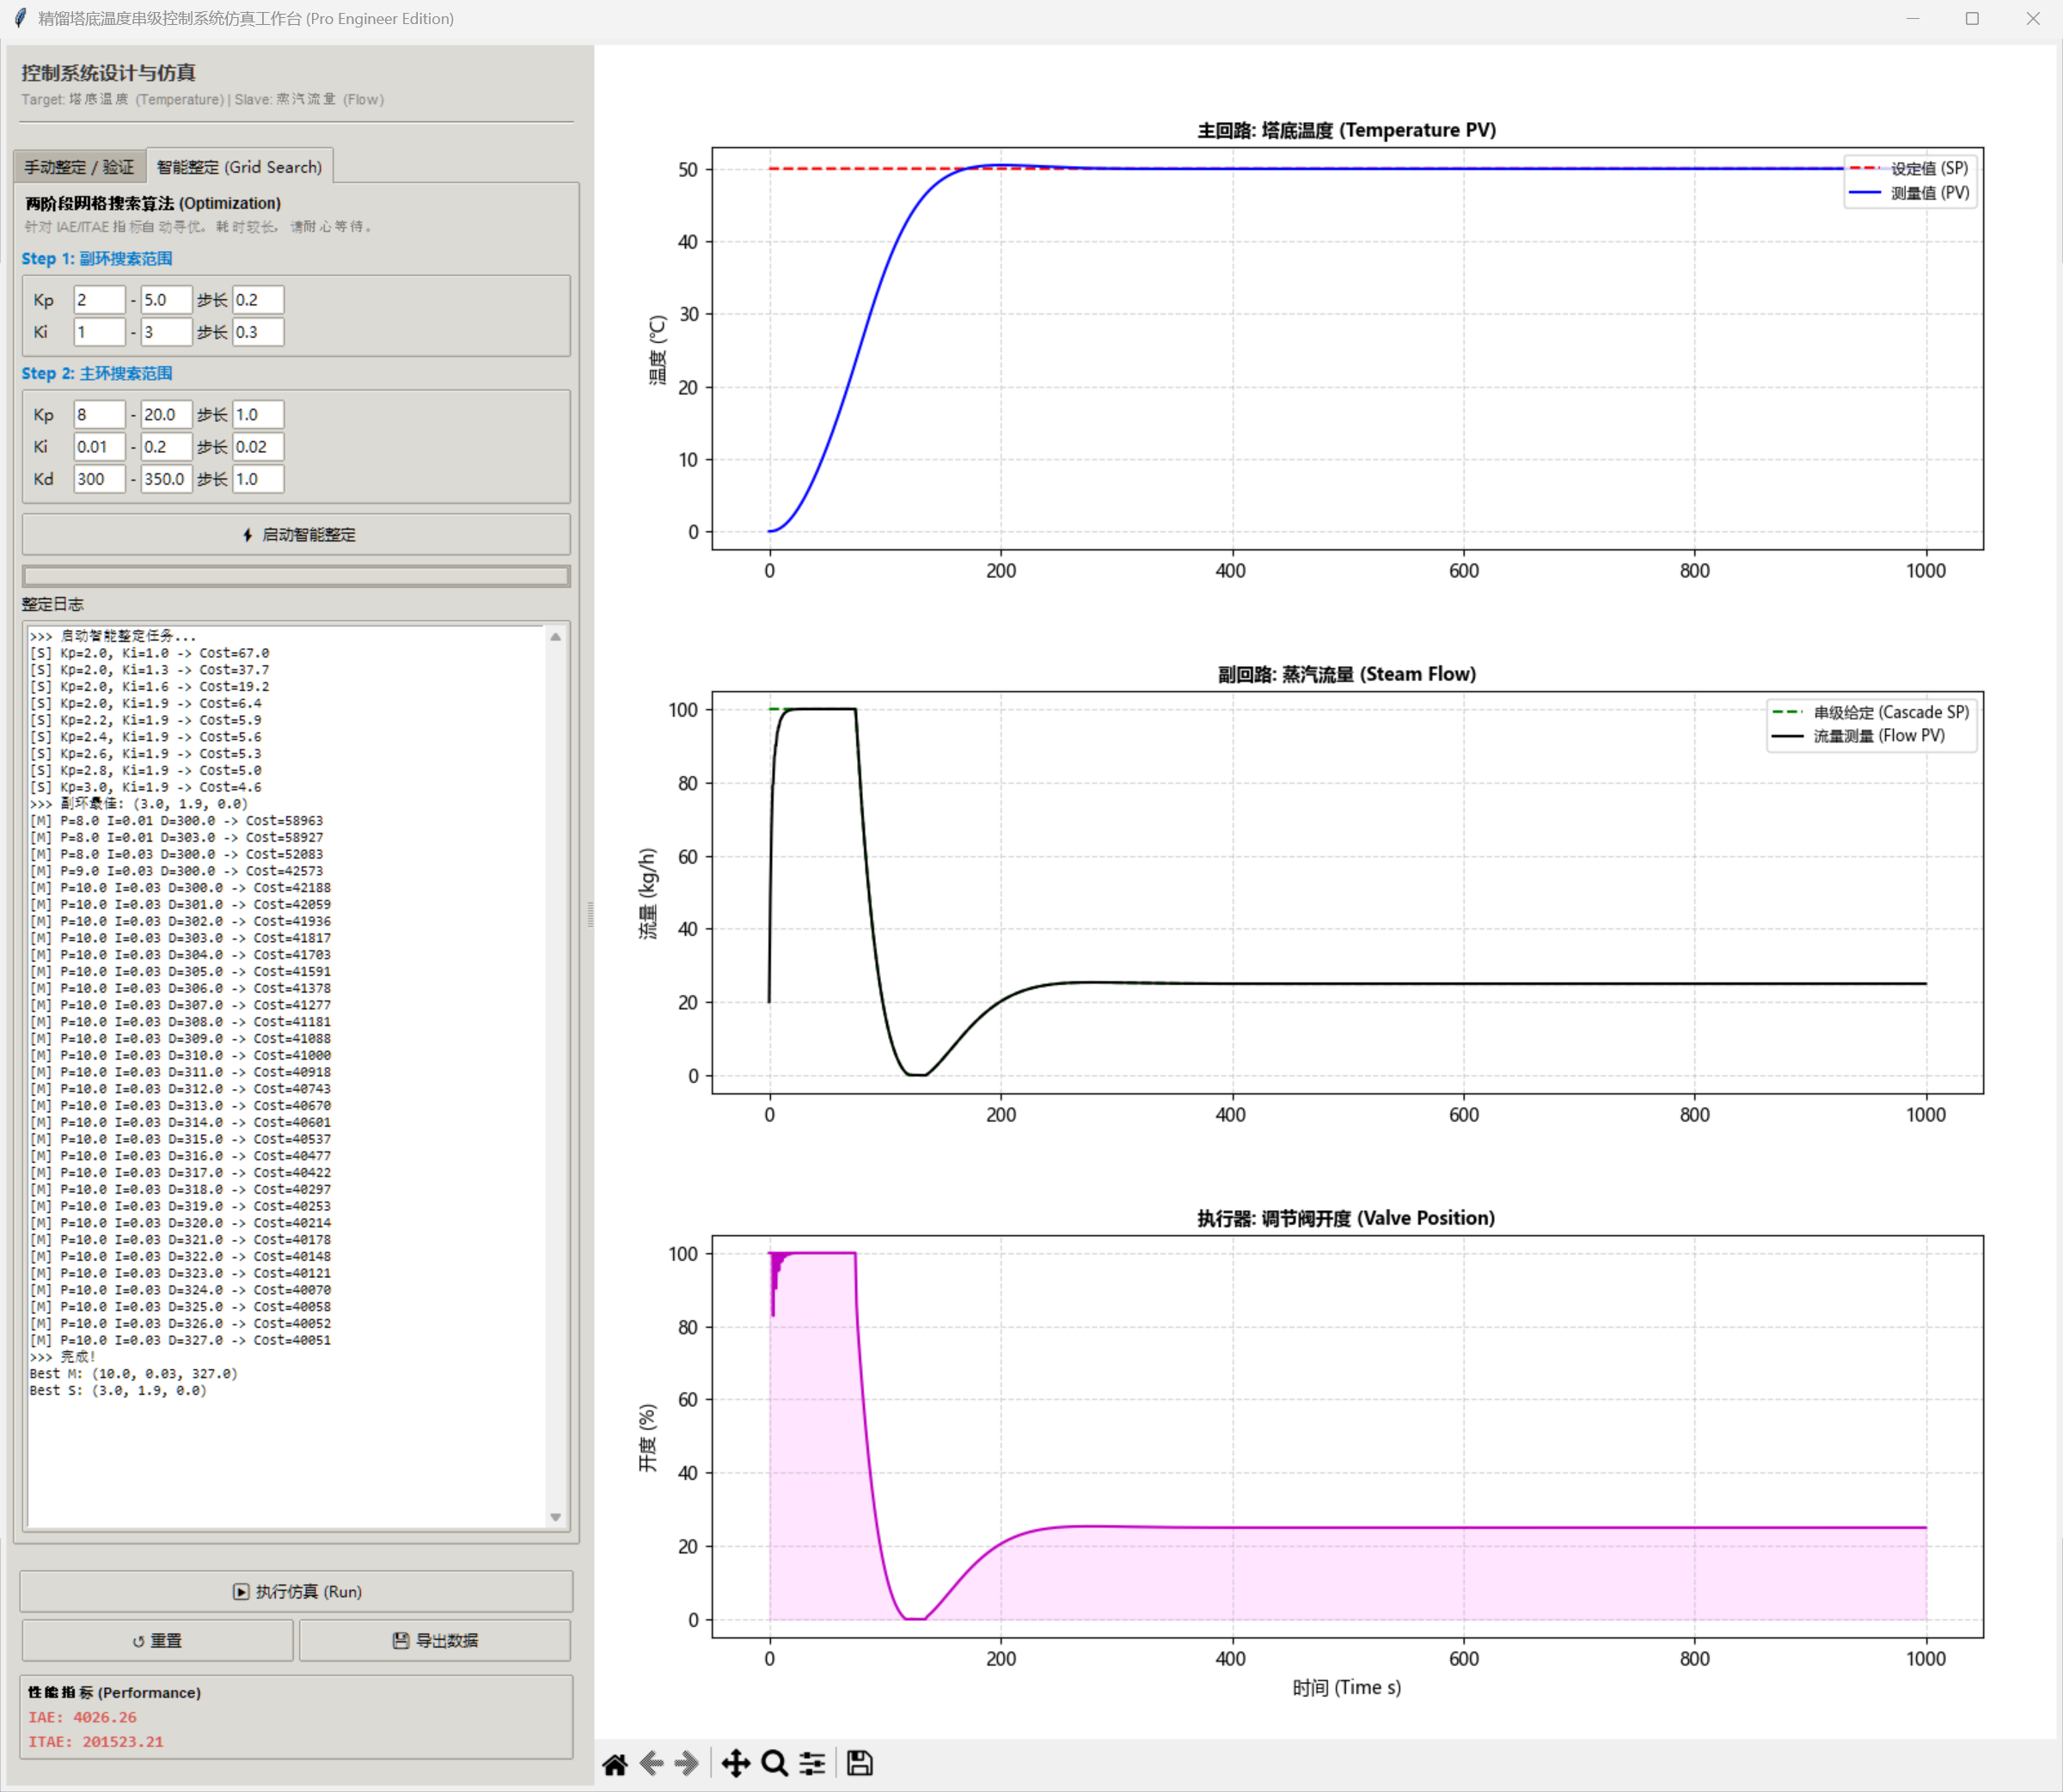
\includegraphics[width=0.95\textwidth]{simulated.png}
	\caption{塔底温度串级控制系统参数整定及仿真响应}
	\label{fig:simulation_result}
\end{figure}

\begin{equation}
	Loss = 
	\begin{cases}
		L_1 + 1, & L_1 > 0 \\
		\Bigl(1 - \frac{1}{J}\Bigr) \cdot e^{-| \max\{\int_{\Omega} j(\theta, x) dx, -1 \} | }, & L_1 = 0
	\end{cases}
\end{equation}
where \begin{equation}
	L_1 = \int_{\Omega} \max \{j(\theta, x) + \varepsilon \|x\|^{2}, 0\}^{2} dx
\end{equation}
\begin{equation}
	j(\theta, x) = L_{f} V_{N}(\theta, \delta, x) - \sum_{i=1}^{m} U_i \left| L_{g_i} V_{N}(\theta, \delta, x) \right|
\end{equation}
积分的计算方法保持不变还是通过配点均匀采样并求和；这里的$J$是性能指标
$J = -\int_{0}^{T} \left( q_1 \theta^2 + q_2 \dot{\theta}^2 + r u^2\right)dt$,
$T$是仿真时长,$q_1=10,q_2=1,r=0.1$,$J$是关于状态变量$x=[\theta,\dot\theta]^T$和控制输入$u$的函数，由于Sontag公式，$u$是状态变量$x$和李函数V的函数，所以把$J$写为$J(x,V)$。其计算方式为在训练过程里每计算出一个李函数V就进行一次仿真并求取一个对应的$J$。在实际中为了节省计算时间，只有在满足$L_1 \leq 1e-8$时才进行仿真并计算$J$，并且所有训练阶段的仿真和性能指标计算均采用前向欧拉法，使用$x(k+1)=\Delta t \cdot (fx(k)+gu)+x(k)$来迭代计算，但是最终完成训练后的仿真验证时还是用原来的龙格库塔方法。。
还将epoch轮数改为100次。同样为了节省计算时间，最开始仿真和计算$J$采用大的时间间隔，比如0.001s，在连续3个epoch里损失函数变化量$\leq 1e-4$后才采取相对精准的仿真，这时在连续5个epoch里损失函数变化量$\leq 1e-5$后早停，训练进入每个epoch和每个阶段都要报告一次，最后可视化保持不变

%---------------------------------------------------------------------------------
% 参考文献
%---------------------------------------------------------------------------------
\newpage
\begin{thebibliography}{99}
	\addcontentsline{toc}{section}{参考文献} % 将参考文献加入目录
	
	\bibitem{1} 佚名. 化工单元操作——精馏塔[EB/OL]. 2023-10-08. \url{https://www.qzlyizjut.com/102244.html}.
	
	\bibitem{2} 荣启工程设计. 精馏塔原理的主要结构[EB/OL]. 2024-07-03. \url{https://mp.weixin.qq.com/s?__biz=Mzg3OTY4NDY1Ng==&mid=2247502573&idx=3&sn=61a619720c8d4406f9b3d1c79c32b260}.
	
	\bibitem{3} 昆明理工大学化学工程学院. 精馏原理[EB/OL]（PPT）. 昆明理工大学化学工程学院教学资源, [出版日期不详]. \url{https://hg.kmust.edu.cn/__local/6/8F/B5/7F1D2201DDF80F1C06230202EDD_97195123_60DD1.pdf?e=.pdf}.
	
	\bibitem{4} 易思在线. 精馏原理[EB/OL]. 易思在线仿真实验平台, 2019-11-05. \url{https://nvse.es-online.com.cn/Uploads/20191105/372ae827-4de6-4cd1-99fa-42bc7ddb2122.pdf}.
	
	\bibitem{5} Juan Gabriel Segovia-Hernández, Salvador Hernández, Eduardo Sánchez-Ramírez, Jesús Mendoza-Pedroza. A Short Review of Dividing Wall Distillation Column as an Application of Process Intensification: Geographical Development and the Pioneering Contribution of Prof. Arturo Jimenez in Latin America[J]. Chemical Engineering and Processing - Process Intensification, 2021, 160: 108275. \url{https://doi.org/10.1016/j.cep.2020.108275}.
	
	\bibitem{6} Ziwei Shen, Qingping Qu, Meili Chen, Hao Lyu, Jinsheng Sun. Advancements in methanol distillation system: A comprehensive overview[J]. Chemical Engineering Research and Design, 2023, 199: 130-151. \url{https://doi.org/10.1016/j.cherd.2023.09.026}.
	
	\bibitem{7} 袁美龙, 胡传伍, 华超, 等. 萃取精馏技术研究及应用进展[J]. 山东化工, 2024, 53(21): 135-138. \url{https://doi.org/10.19319/j.cnki.issn.1008-021x.2024.21.043}.
	
	\bibitem{8} 张敏. 聚乙烯醇副产物醋酸甲酯提纯工艺研究进展[J]. 山东化工, 2015, 44(15): 76-77+79. \url{https://doi.org/10.19319/j.cnki.issn.1008-021x.2015.15.031}.
	
\end{thebibliography}
\end{document}